\newpage
\section*{Appendix}
We include several appendices with additional details, derivations, and results.
Our framework allows general SDEs with matrix-valued diffusion coefficients that depend on the state, for which we provide a detailed discussion in \cref{app:general_sde}. We give a full derivation of VE and VP SDEs in \cref{app:sde_derive}, and discuss how to use them from a practitioner's perspective in \cref{app:wild_sde}. We elaborate on the probability flow formulation of our framework in \cref{app:prob_flow_ode}, including a derivation of the probability flow ODE (\cref{app:prob_flow_derive}), exact likelihood computation (\cref{app:prob_flow_likelihood}), probability flow sampling (\cref{app:prob_flow_sampling,app:flow}) and experimental verification on uniquely identifiable encoding (\cref{app:identifiability}). We give a full description of the reverse diffusion sampler in \cref{app:reverse_diffusion}, and the DDPM-type ancestral sampler for SMLD models in \cref{app:ancestral}. We provide full experimental details on Predictor-Corrector samplers in \cref{app:pc}. We explain our model architectures and detailed experimental settings in \cref{app:arch_search}, with $1024\times 1024$ CelebA-HQ samples therein. Finally, we detail on the algorithms for controllable generation in \cref{app:cond_gen}, and include extended results for class-conditional generation (\cref{app:class_cond_sampling}), image inpainting (\cref{app:imputation}) and colorization (\cref{app:colorization}).

\section{The framework for more general SDEs}\label{app:general_sde}
In the main text, we introduced our framework based on a simplified SDE~\cref{eqn:forward_sde} where the diffusion coefficient is independent of $\bfx(t)$. It turns out that our framework can be extended to hold for more general diffusion coefficients. We can consider SDEs in the following form:
\begin{align}
    \ud \bfx = \bff(\bfx, t) \ud t + \mbf{G}(\bfx, t) \ud \bfw, \label{eqn:forward_sde_2}
\end{align}
where $\bff(\cdot, t): \mbb{R}^d \to \mbb{R}^d$ and $\mbf{G}(\cdot, t): \mbb{R}^d \to \mbb{R}^{d\times d}$. We follow the It\^{o} interpretation of SDEs throughout this paper.

According to \citep{Anderson1982-ny}, the reverse-time SDE is given by (\cf, \cref{eqn:backward_sde})
\begin{align}
    \ud \bfx = \{\bff(\bfx, t) - \nabla \cdot [\bfG(\bfx, t) \bfG(\bfx,t)\tran] - \bfG(\bfx,t)\bfG(\bfx,t)\tran  \nabla_\bfx  \log p_t(\bfx)\} \ud t + \mbf{G}(\bfx, t) \ud \bar{\bfw},\label{eqn:backward_sde_2}
\end{align}
where we define $\nabla\cdot \mbf{F}(\bfx) := (\nabla \cdot \bff^1(\bfx), \nabla\cdot \bff^2(\bfx), \cdots, \nabla\cdot \bff^d(\bfx))\tran$ for a matrix-valued function $\mbf{F}(\bfx) := (\bff^1(\bfx), \bff^2(\bfx), \cdots, \bff^d(\bfx))\tran$ throughout the paper. 

The probability flow ODE corresponding to \cref{eqn:forward_sde_2} has the following form (\cf, \cref{eqn:flow}, see a detailed derivation in \cref{app:prob_flow_derive}):
\begin{align}
    \ud \bfx = \bigg\{\bff(\bfx, t) - \frac{1}{2} \nabla \cdot [\bfG(\bfx, t)\bfG(\bfx, t)\tran] - \frac{1}{2} \bfG(\bfx, t)\bfG(\bfx, t)\tran \nabla_\bfx \log p_t(\bfx)\bigg\} \ud t. \label{eqn:flow_2}
\end{align}
Finally for conditional generation with the general SDE \cref{eqn:forward_sde_2}, we can solve the conditional reverse-time SDE below (\cf, \cref{eqn:cond_sde}, details in \cref{app:cond_gen}):
\begin{multline}
\ud \bfx = \{\bff(\bfx, t) - \nabla \cdot [\bfG(\bfx, t) \bfG(\bfx,t)\tran] - \bfG(\bfx,t)\bfG(\bfx,t)\tran  \nabla_\bfx  \log p_t(\bfx)\\ - \bfG(\bfx,t)\bfG(\bfx,t)\tran  \nabla_{\bfx}  \log p_t(\bfy \mid \bfx)\} \ud t + \mbf{G}(\bfx, t) \ud \bar{\bfw}.\label{eqn:cond_sde_2}
\end{multline}

When the drift and diffusion coefficient of an SDE are not affine, it can be difficult to compute the transition kernel $p_{0t}(\bfx(t) \mid \bfx(0))$ in closed form. This hinders the training of score-based models, because \cref{eqn:training} requires knowing $\nabla_{\bfx(t)}\log p_{0t}(\bfx(t) \mid \bfx(0))$. To overcome this difficulty, we can replace denoising score matching in \cref{eqn:training} with other efficient variants of score matching that do not require computing $\nabla_{\bfx(t)}\log p_{0t}(\bfx(t) \mid \bfx(0))$. For example, when using sliced score matching~\citep{song2019sliced}, our training objective \cref{eqn:training} becomes
\begin{align}
   \bftheta^* = \argmin_\bftheta 
   \mbb{E}_{t}\bigg\{\lambda(t) \mbb{E}_{\bfx(0)}\mbb{E}_{\bfx(t) }\mbb{E}_{\bfv \sim p_\bfv}
   \bigg[\frac{1}{2}\norm{\bfs_\bftheta(\bfx(t), t)}_2^2 + \bfv\tran \bfs_\bftheta(\bfx(t), t) \bfv \bigg]\bigg\}%
   , \label{eqn:training_ssm}
\end{align}
where $\lambda: [0,T] \to \mbb{R}^+$ is a positive weighting function, $t \sim \mcal{U}(0, T)$, $\mbb{E}[\bfv] = \bfzero$, and $\operatorname{Cov}[\bfv] = \bfI$. We can always simulate the SDE to sample from $p_{0t}(\bfx(t) \mid \bfx(0))$, and solve \cref{eqn:training_ssm} to train the time-dependent score-based model $\bfs_\bftheta(\bfx, t)$.




\section{Derivations of VE and VP SDEs}\label{app:sde_derive}
Below we provide detailed derivations to show that the noise perturbations of SMLD and DDPM are discretizations of the Variance Exploding (VE) and Variance Preserving (VP) SDEs respectively.

First, when using a total of $N$ noise scales, each perturbation kernel $p_{\sigma_i}(\bfx \mid \bfx_0)$ of SMLD can be derived from the following Markov chain:
\begin{align}
\bfx_i = \bfx_{i-1} + \sqrt{\sigma_{i}^2 - \sigma_{i-1}^2} \bfz_{i-1}, \quad i=1,\cdots,N \label{eqn:ncsn},
\end{align}
where $\bfz_{i-1} \sim \mcal{N}(\bfzero, \bfI)$, $\bfx_0 \sim p_\text{data}$, and we have introduced $\sigma_0 = 0$ to simplify the notation.
In the limit of $N \to \infty$, the Markov chain $\{\bfx_i\}_{i=1}^N$ becomes a continuous stochastic process $\{\bfx(t)\}_{t=0}^1$, $\{\sigma_i\}_{i=1}^N$ becomes a function $\sigma(t)$, and $\bfz_i$ becomes $\bfz(t)$, where we have used a continuous time variable $t \in [0, 1]$ for indexing, rather than an integer $i \in \{1, 2, \cdots, N\}$. 
Let $\bfx\left(\frac{i-1}{N-1}\right) = \bfx_i$, $\sigma\left(\frac{i-1}{N-1}\right) = \sigma_i$, and $\bfz\left(\frac{i-1}{N-1}\right) = \bfz_i$ for $i=1,2,\cdots, N$. We can rewrite \cref{eqn:ncsn} as follows with $\Delta t = \frac{1}{N-1}$ and $t \in \big\{0, \frac{1}{N-1}, \cdots, \frac{N-2}{N-1}\big\}$:
\begin{align*}
    \bfx(t + \Delta t) = \bfx(t) + \sqrt{\sigma^2(t + \Delta t)- \sigma^2(t)}~\bfz(t) \approx \bfx(t) + \sqrt{\frac{\ud \left[ \sigma^2(t) \right] }{\ud t}\Delta t} ~\bfz(t),
\end{align*}
where the approximate equality holds when $\Delta t \ll 1$. 
In the limit of $\Delta t \rightarrow 0$, this converges to
\begin{align}
\ud \bfx = \sqrt{\frac{\ud \left[ \sigma^2(t) \right]}{\ud t}}\ud \bfw, \label{eqn:ncsn_sde_2}
\end{align}
which is the VE SDE. Note that $\bfx(0) = \bfx_1 = \bfx_0 + \sigma_1 \bfz_0 = \bfx_0 + \sigma^2(0) \bfz_0$ and $\bfx_0 \sim p_\text{data}$, so we have $p_0(\bfx(0)) = \int p_\text{data}(\bfx) \mcal{N}(\bfx(0); \bfx, \sigma_1^2 \bfI) \ud \bfx$. In other words, $p_0(\bfx(0))$ for the VE SDE is a perturbed data distribution with a small Gaussian noise.

For the perturbation kernels $\{p_{\alpha_i}(\bfx \mid \bfx_0)\}_{i=1}^N$ used in DDPM, the discrete Markov chain is
\begin{align}
    \bfx_i = \sqrt{1-\beta_{i}} \bfx_{i-1} + \sqrt{\beta_{i}} \bfz_{i-1}, \quad i=1,\cdots,N, \label{eqn:ddpm_markov}
\end{align}
where $\bfz_{i-1} \sim \mcal{N}(\bfzero, \bfI)$. To obtain the limit of this Markov chain when $N\to\infty$, we define an auxiliary set of noise scales $\{\bbeta_i = N \beta_i\}_{i=1}^N$, and re-write \cref{eqn:ddpm_markov} as below
\begin{align}
    \bfx_i = \sqrt{1-\frac{\bbeta_{i}}{N}} \bfx_{i-1} + \sqrt{\frac{\bbeta_{i}}{N}} \bfz_{i-1}, \quad i=1,\cdots,N. \label{eqn:ddpm_markov2}
\end{align}
In the limit of $N\to \infty$, $\{\bbeta_i\}_{i=1}^N$ becomes a function $\beta(t)$ indexed by $t \in [0, 1]$. Let $\beta\left(\frac{i}{N}\right) = \bbeta_i$, $\bfx(\frac{i}{N}) = \bfx_i$, $\bfz(\frac{i}{N}) = \bfz_i$. We can rewrite the Markov chain \cref{eqn:ddpm_markov2} as the following with $\Delta t = \frac{1}{N}$ and $t \in \{0, 1, \cdots, \frac{N-1}{N}\}$:
\begin{align}
\bfx(t + \Delta t) &= \sqrt{1 - \beta(t + \Delta t)\Delta t} ~\bfx(t) + \sqrt{\beta(t + \Delta t)\Delta t}~ \bfz(t) \notag\\
&\approx -\frac{1}{2}\beta(t)\Delta t~\bfx(t) + \sqrt{\beta(t)\Delta t}~ \bfz(t), \label{eqn:ddpm_discrete}
\end{align}
where the approximate equality holds when $\Delta t \ll 1$.
Therefore, in the limit of $\Delta t \to 0$, \cref{eqn:ddpm_discrete} converges to the following VP SDE:
\begin{align}
\ud \bfx = -\frac{1}{2}\beta(t) \bfx~ \ud t + \sqrt{\beta(t)} ~\ud \bfw.
\end{align}
Since $\bfx(0) = \bfx_0$ and $\bfx_0 \sim p_\text{data}$, we have $p_0(\bfx(0)) = p_\text{data}(\bfx)$.

So far, we have demonstrated that the noise perturbations used in SMLD and DDPM correspond to discretizations of VE and VP SDEs respectively. The VE SDE always yields a process with exploding variance when $t \to \infty$. In contrast, the VP SDE yields a process with bounded variance. In addition, the process has a constant unit variance for all $t \in [0, \infty)$ when $p(\bfx(0))$ has a unit variance. Since the VP SDE has affine drift and diffusion coefficients, we can use Eq.~(5.51) in \citet{sarkka2019applied} to obtain an ODE that governs the evolution of variance
\begin{align*}
    \frac{\ud \bfsigma(t)}{\ud t} = \beta(t) (\bfI - \bfsigma(t)),
\end{align*}
where $\bfsigma(t) = \operatorname{Cov}[\bfx(t)]$. Solving this ODE, we obtain
\begin{align*}
    \bfsigma(t) = \bfI + e^{\int_0^T - \beta(t) \ud t}(\bfsigma(0) - \bfI),
\end{align*}
from which it is clear that the variance $\bfsigma(t)$ is always bounded given $\bfsigma(0)$. Moreover, $\bfsigma(t) \equiv \bfI$ if $\bfsigma(0) = \bfI$. Due to this difference, we name \cref{eqn:ncsn_sde} as the \emph{Variance Exploding (VE) SDE}, and \cref{eqn:ddpm_sde} the \emph{Variance Preserving (VP) SDE}.

Since both VE and VP SDEs have affine drift coefficients, their perturbation kernels $p_{0t}(\bfx(t) \mid \bfx(0))$ are both Gaussian and can be computed with Eqs.~(5.50) and (5.51) in \citet{sarkka2019applied}:
\begin{align}
    p_{0t}(\bfx(t) \mid \bfx(0)) = \begin{cases} 
    \mcal{N}\big(\bfx(t) ; \bfx(0), [\sigma^2(t) - \sigma^2(0)] \bfI\big), &~~~ \text{(VE SDE)}\\
    \mcal{N}\big(\bfx(t) ; \bfx(0)e^{-\frac{1}{2}\int_0^t \beta(s) \ud s}, \bfI - \bfI e^{-\int_0^t \beta(s) \ud s}\big) &~~~ \text{(VP SDE)} 
    \end{cases}.\label{eqn:perturb_kernel}
\end{align}
Therefore, both SDEs allow efficient training with the objective in \cref{eqn:training}.

\section{SDEs in the wild} \label{app:wild_sde}
Below we discuss SDEs that directly correspond to implementations for practical SMLD and DDPM models. In SMLD, the noise scales $\{\sigma_i\}_{i=1}^N$ is typically a geometric sequence where $\sigma_\text{min}$ is fixed to $0.01$ and $\sigma_\text{max}$ is chosen according to Technique 1 in \citet{song2020improved}. Usually, SMLD models normalize image inputs to the range $[0, 1]$. Since $\{\sigma_i\}_{i=1}^N$ is a geometric sequence, we have $\sigma_i = \sm \left(\frac{\sM}{\sm}\right)^{\frac{i-1}{N-1}}$ and therefore $\sigma(t) = \sm \left(\frac{\sM}{\sm}\right)^{t}$. The VE SDE in this case is
\begin{align}
\ud \bfx = \sm \bigg( \frac{\sM}{\sm} \bigg)^t \sqrt{2 \log \frac{\sM}{\sm}}\ud \bfw,
\end{align}
where $\bfx(0) \sim \int p_\text{data}(\bfx) \mcal{N}(\bfx(0); \bfx, \sm^2 \bfI) \ud \bfx$. The perturbation kernel can be computed via \cref{eqn:perturb_kernel}:
\begin{align}
    p_{0t}(\bfx(t) \mid \bfx(0)) = \mcal{N}\left(\bfx(t) ; \bfx(0), \Big[\sm^2 \Big( \frac{\sM}{\sm}\Big)^{2t} - \sm^2\Big] \bfI\right).
\end{align}
Since $\bfx(0) \sim \mcal{N}(\bfx_0, \sm^2 \bfI)$ and $\bfx_0 \sim p_\text{data}(\bfx)$, we also have
\begin{align*}
    p_{0t}(\bfx(t) \mid \bfx_0) = \mcal{N}\left(\bfx(t) ; \bfx(0), \sm^2 \Big( \frac{\sM}{\sm}\Big)^{2t} \bfI\right).
\end{align*}

For DDPM models, $\{\beta_i\}_{i=1}^N$ is typically an arithmetic sequence where $\beta_i = \frac{\bbetam}{N-1} + \frac{i-1}{(N-1)^2}(\bbetaM -\bbetam)$. Therefore, $\beta(t) = \bbetam + t(\bbetaM - \bbetam)$. This corresponds to the following instantiation of the VP SDE:
\begin{gather}
\ud \bfx = -\frac{1}{2}(\bbetam + t(\bbetaM - \bbetam)) \bfx \ud t + \sqrt{\bbetam + t(\bbetaM - \bbetam)} \ud \bfw,
\end{gather}
where $\bfx(0) \sim p_\text{data}(\bfx)$. In our experiments, we let $\bbetam = 0.1$ and $\bbetaM = 20$, which correspond to the settings in \citet{ho2020denoising}. The perturbation kernel is given by
\begin{align}
    p_{0t}(\bfx(t) \mid \bfx(0)) = \mcal{N}\left(\bfx(t) ; e^{-\frac{1}{4}t^2(\bbetaM-\bbetam) - \frac{1}{2}t\bbetam}\bfx(0), \bfI - \bfI e^{-\frac{1}{2}t^2(\bbetaM -\bbetam) - t\bbetam} \right).
\end{align}

\begin{figure}
    \centering
    \begin{subfigure}{0.333\linewidth}
        \includegraphics[width=\linewidth]{figures/NCSN_var.pdf}%
        \caption{SMLD}
    \end{subfigure}
    \begin{subfigure}{0.32\linewidth}
        \includegraphics[width=\linewidth]{figures/ddpm_mean.pdf}%
        \caption{DDPM (mean)}
    \end{subfigure}
    \begin{subfigure}{0.32\linewidth}
        \includegraphics[width=\linewidth]{figures/ddpm_var.pdf}
        \caption{DDPM (variance)}
    \end{subfigure}
    \caption{Discrete-time perturbation kernels and our continuous generalizations match each other almost exactly. (a) compares the variance of perturbation kernels for SMLD and VE SDE; (b) compares the scaling factors of means of perturbation kernels for DDPM and VP SDE; and (c) compares the variance of perturbation kernels for DDPM and VP SDE.}
    \label{fig:discretization}
\end{figure}
As a sanity check for our SDE generalizations to SMLD and DDPM, we compare the perturbation kernels of SDEs and original discrete Markov chains in \cref{fig:discretization}. The SMLD and DDPM models both use $N=1000$ noise scales. For SMLD, we only need to compare the variances of perturbation kernels. For DDPM, we compare the scaling factors of means and the variances. As demonstrated in \cref{fig:discretization}, the discrete perturbation kernels of original SMLD and DDPM models align well with perturbation kernels derived from VE and VP SDEs.


\section{Probability flow ODE}\label{app:prob_flow_ode}
\subsection{Derivation}\label{app:prob_flow_derive}
The idea of probability flow ODE is inspired by \citet{maoutsa2020interacting}, and one can find the derivation of a simplified case therein. Below we provide a derivation for the fully general ODE in \cref{eqn:flow_2}. We consider the SDE in \cref{eqn:forward_sde_2}, which possesses the following form:
\begin{align*}
    \ud \bfx = \bff(\bfx, t) \ud t + \mbf{G}(\bfx, t) \ud \bfw,
\end{align*}
where $\bff(\cdot, t): \mbb{R}^d \to \mbb{R}^d$ and $\mbf{G}(\cdot, t): \mbb{R}^d \to \mbb{R}^{d\times d}$. The marginal probability density $p_t(\mbf{x}(t))$ evolves according to the forward Kolmogorov equation (Fokker-Planck equation)~\citep{oksendal2003stochastic}
\begin{align}
    \frac{\partial p_t(\bfx)}{\partial t} = -\sum_{i=1}^d \frac{\partial}{\partial x_i}[f_i(\bfx, t) p_t(\bfx)] + \frac{1}{2}\sum_{i=1}^d\sum_{j=1}^d \frac{\partial^2}{\partial x_i \partial x_j}\Big[\sum_{k=1}^d G_{ik}(\bfx, t) G_{jk}(\bfx, t) p_t(\bfx)\Big] \label{eqn:fokker_planck}.
\end{align}
We can easily rewrite \cref{eqn:fokker_planck} to obtain
\begin{align}
    \frac{\partial p_t(\bfx)}{\partial t} &= -\sum_{i=1}^d \frac{\partial}{\partial x_i}[f_i(\bfx, t) p_t(\bfx)] + \frac{1}{2}\sum_{i=1}^d\sum_{j=1}^d \frac{\partial^2}{\partial x_i \partial x_j}\Big[\sum_{k=1}^d G_{ik}(\bfx, t) G_{jk}(\bfx, t) p_t(\bfx)\Big]\notag \\
    &= -\sum_{i=1}^d \frac{\partial}{\partial x_i}[f_i(\bfx, t) p_t(\bfx)] + \frac{1}{2}\sum_{i=1}^d \frac{\partial}{\partial x_i} \Big[ \sum_{j=1}^d \frac{\partial}{\partial x_j}\Big[\sum_{k=1}^d G_{ik}(\bfx, t) G_{jk}(\bfx, t) p_t(\bfx)\Big]\Big]. \label{eqn:ode_part_1}
\end{align}
Note that
\begin{align*}
    &\sum_{j=1}^d \frac{\partial}{\partial x_j}\Big[\sum_{k=1}^d G_{ik}(\bfx, t) G_{jk}(\bfx, t) p_t(\bfx)\Big]\\
    =& \sum_{j=1}^d \frac{\partial}{\partial x_j} \Big[ \sum_{k=1}^d G_{ik}(\bfx, t) G_{jk}(\bfx, t) \Big] p_t(\bfx) + \sum_{j=1}^d \sum_{k=1}^d G_{ik}(\bfx, t)G_{jk}(\bfx, t) p_t(\bfx) \frac{\partial}{\partial x_j} \log p_t(\bfx)\\
    =& p_t(\bfx) \nabla \cdot [\bfG(\bfx, t)\bfG(\bfx, t)\tran] + p_t(\bfx) \bfG(\bfx, t)\bfG(\bfx, t)\tran \nabla_\bfx \log p_t(\bfx),
\end{align*}
based on which we can continue the rewriting of \cref{eqn:ode_part_1} to obtain
\begin{align}
    \frac{\partial p_t(\bfx)}{\partial t} &= -\sum_{i=1}^d \frac{\partial}{\partial x_i}[f_i(\bfx, t) p_t(\bfx)] + \frac{1}{2}\sum_{i=1}^d \frac{\partial}{\partial x_i} \Big[ \sum_{j=1}^d \frac{\partial}{\partial x_j}\Big[\sum_{k=1}^d G_{ik}(\bfx, t) G_{jk}(\bfx, t) p_t(\bfx)\Big]\Big]\notag \\
     &= -\sum_{i=1}^d \frac{\partial}{\partial x_i}[f_i(\bfx, t) p_t(\bfx)] \notag \\
     &\quad + \frac{1}{2}\sum_{i=1}^d \frac{\partial}{\partial x_i} \Big[ p_t(\bfx) \nabla \cdot [\bfG(\bfx, t)\bfG(\bfx, t)\tran] + p_t(\bfx) \bfG(\bfx, t)\bfG(\bfx, t)\tran \nabla_\bfx \log p_t(\bfx) \Big]\notag \\
     &= -\sum_{i=1}^d \frac{\partial}{\partial x_i}\Big\{ f_i(\bfx, t)p_t(\bfx) \notag \\
     &\quad - \frac{1}{2} \Big[ \nabla \cdot [\bfG(\bfx, t)\bfG(\bfx, t)\tran] +  \bfG(\bfx, t)\bfG(\bfx, t)\tran \nabla_\bfx \log p_t(\bfx) \Big] p_t(\bfx) \Big\}\notag \\
     &= -\sum_{i=1}^d \frac{\partial}{\partial x_i} [\tilde{f}_i(\bfx, t)p_t(\bfx)],\label{eqn:ode_part_2}
\end{align}
where we define
\begin{align*}
    \tilde{\bff}(\bfx, t) \triangleq \bff(\bfx, t) - \frac{1}{2} \nabla \cdot [\bfG(\bfx, t)\bfG(\bfx, t)\tran] - \frac{1}{2} \bfG(\bfx, t)\bfG(\bfx, t)\tran \nabla_\bfx \log p_t(\bfx).
\end{align*}
Inspecting \cref{eqn:ode_part_2}, we observe that it equates the forward Kolmogorov equation of the following SDE with $\tilde{\bfG}(\bfx, t) \triangleq \bfzero$ (the forward Kolmogorov equation holds in this case, according to the Liouville equation.)
\begin{align*}
    \ud \bfx = \tilde{\bff}(\bfx, t) \ud t + \tilde{\bfG}(\bfx, t) \ud \bfw,
\end{align*}
which is essentially an ODE:
\begin{align*}
    \ud \bfx = \tilde{\bff}(\bfx, t) \ud t,
\end{align*}
same as the probability flow ODE given by \cref{eqn:flow_2}. Therefore, we have shown that the probability flow ODE \cref{eqn:flow_2} induces the same marginal probability density $p_t(\bfx)$ as the SDE in \cref{eqn:forward_sde_2}.

\subsection{Likelihood computation}\label{app:prob_flow_likelihood}
The probability flow ODE in \cref{eqn:flow_2} has the following form when we replace the score $\nabla_\bfx \log p_t(\bfx)$ with the time-dependent score-based model $\bfs_\bftheta(\bfx, t)$:
\begin{align}
      \ud \bfx = \underbrace{\bigg\{\bff(\bfx, t) - \frac{1}{2} \nabla \cdot [\bfG(\bfx, t)\bfG(\bfx, t)\tran] - \frac{1}{2} \bfG(\bfx, t)\bfG(\bfx, t)\tran \bfs_\bftheta(\bfx, t)\bigg\}}_{\triangleq \tilde{\bff}_\bftheta(\bfx, t)} \ud t. \label{eqn:flow_3}
\end{align}
With the instantaneous change of variables formula~\citep{chen2018neural}, we can compute the log-likelihood of $p_0(\bfx)$ using
\begin{align}
    \log p_0(\bfx(0)) = \log p_T(\bfx(T)) + \int_0^T \nabla \cdot \tilde{\bff}_\bftheta(\bfx(t), t) \ud t, \label{eqn:likelihood}
\end{align}
where the random variable $\bfx(t)$ as a function of $t$ can be obtained by solving the probability flow ODE in \cref{eqn:flow_3}. In many cases computing $\nabla \cdot \tilde{\bff}_\bftheta(\bfx, t)$ is expensive, so we follow \citet{grathwohl2018ffjord} to estimate it with the Skilling-Hutchinson trace estimator~\citep{skilling1989eigenvalues,hutchinson1990stochastic}. In particular, we have
\begin{align}
    \nabla \cdot \tilde{\bff}_\bftheta(\bfx, t) = \mbb{E}_{p(\bfe)}[\bfe\tran \nabla \tilde{\bff}_\bftheta(\bfx, t)\bfe], \label{eqn:hutchinson}
\end{align}
where $\nabla \tilde{\bff}_\bftheta$ denotes the Jacobian of $\tilde{\bff}_\bftheta(\cdot, t)$, and the random variable $\bfe$ satisfies $\mbb{E}_{p(\bfe)}[\bfe] = \bfzero$ and $\operatorname{Cov}_{p(\bfe)}[\bfe] = \bfI$. The vector-Jacobian product $\bfe\tran \nabla\tilde{\bff}_\bftheta(\bfx, t)$ can be efficiently computed using reverse-mode automatic differentiation, at approximately the same cost as evaluating $\tilde{\bff}_\bftheta(\bfx, t)$. As a result, we can sample $\bfe \sim p(\bfe)$ and then compute an efficient unbiased estimate to $\nabla \cdot \tilde{\bff}_\bftheta(\bfx, t)$ using $\bfe\tran \nabla \tilde{\bff}_\bftheta(\bfx, t) \bfe$. Since this estimator is unbiased, we can attain an arbitrarily small error by averaging over a sufficient number of runs. Therefore, by applying the Skilling-Hutchinson estimator \cref{eqn:hutchinson} to \cref{eqn:likelihood}, we can compute the log-likelihood to any accuracy.


\subsection{Probability flow sampling}\label{app:prob_flow_sampling}
Suppose we have a forward SDE
\begin{align*}
    \ud \bfx = \bff(\bfx, t) \ud t + \bfG(t) \ud \bfw,
\end{align*}
and one of its discretization
\begin{align}
    \bfx_{i+1} = \bfx_i + \bff_i(\bfx_i) + \bfG_i \bfz_i, \quad i = 0, 1, \cdots, N-1, \label{eqn:discrete_forward_2}
\end{align}
where $\bfz_i \sim \mcal{N}(\bfzero, \bfI)$. We assume the discretization schedule of time is fixed beforehand, and thus we absorb the dependency on $\Delta t$ into the notations of $\bff_i$ and $\bfG_i$. Using \cref{eqn:flow_2}, we can obtain the following probability flow ODE:
\begin{align}
    \ud \bfx = \left\{ \bff(\bfx, t) - \frac{1}{2}\bfG(t)\bfG(t)\tran \nabla_\bfx \log p_t(\bfx) \right\} \ud t.
\end{align}
We may employ any numerical method to integrate the probability flow ODE backwards in time for sample generation. In particular, we propose a discretization in a similar functional form to \cref{eqn:discrete_forward_2}:
\begin{align*}
    \bfx_i = \bfx_{i+1} - \bff_{i+1}(\bfx_{i+1}) + \frac{1}{2}\bfG_{i+1}\bfG_{i+1}\tran \bfs_{\bftheta^*}(\bfx_{i+1}, i+1),\quad  i =0,1,\cdots, N-1,
\end{align*}
where the score-based model $\bfs_{\bftheta^*}(\bfx_i, i)$ is conditioned on the iteration number $i$. This is a deterministic iteration rule. Unlike reverse diffusion samplers or ancestral sampling, there is no additional randomness once the initial sample $\bfx_N$ is obtained from the prior distribution. When applied to SMLD models, we can get the following iteration rule for probability flow sampling:
\begin{align}
    \bfx_i = \bfx_{i+1} + \frac{1}{2} (\sigma_{i+1}^2 - \sigma_i^2) \bfs_{{\bftheta^*}}(\bfx_{i+1}, \sigma_{i+1}), \quad i=0,1,\cdots, N-1.
\end{align}
Similarly, for DDPM models, we have
\begin{align}
    \bfx_i = (2 - \sqrt{1 -\beta_{i+1}})\bfx_{i+1} + \frac{1}{2} \beta_{i+1} \bfs_{\bftheta^*}(\bfx_{i+1}, i+1), \quad i=0,1,\cdots, N-1.
\end{align}

\subsection{Probability flow sampling with black-box ODE solvers}\label{app:flow}
For producing figures in \cref{fig:prob_flow}, we use a DDPM model trained on $256\times 256$ CelebA-HQ with the same settings in \citet{ho2020denoising}. We use the RK45 ODE solver~\citep{dormand1980family} provided by \verb|scipy.integrate.solve_ivp| in all cases. The bits/dim values in \cref{tab:bpd} are computed with \verb|atol=1e-5| and \verb|rtol=1e-5|, same as \citet{grathwohl2018ffjord}. To give the results for DDPM (probability flow) and DDPM cont. (probability flow) in \cref{tab:bpd}, we average the bits/dim obtained on the test dataset over five different runs. The standard deviation is below $0.005$ for both of them. FID scores are computed on samples from the probability flow sampler.

Aside from the interpolation results in \cref{fig:prob_flow}, we demonstrate more examples of latent space manipulation in \cref{fig:celeba256}, including interpolation and temperature scaling. The model tested here is a DDPM model trained with the same settings in \citet{ho2020denoising}.
\begin{figure}
    \centering
    \includegraphics[width=\linewidth]{figures/celeba_interp.png}
    \includegraphics[width=\linewidth]{figures/celeba_temp.png}
    \caption{Samples from the probability flow ODE on $256\times 256$ CelebA-HQ with VP perturbations. Top: spherical interpolations between random samples. Bottom: temperature rescaling (reducing norm of embedding).}
    \label{fig:celeba256}
\end{figure}

\subsection{Uniquely identifiable encoding}\label{app:identifiability}

\begin{figure}
    \centering
    \includegraphics[width=\linewidth]{figures/identifiability.pdf}
    \caption{Comparing the first 100 dimensions of the latent code obtained for a random CIFAR-10 image. ``Model A'' and ``Model B'' are separately trained with different architectures.}
    \label{fig:identifiability}
\end{figure}

\begin{figure}
    \centering
    \includegraphics[width=0.5\linewidth]{figures/identifiability_boxplot.pdf}
    \includegraphics[width=0.41\linewidth]{figures/identifiability_cor.pdf}
    \caption{\emph{Left}: The dimension-wise difference between encodings obtained by Model A and B. As a baseline, we also report the difference between shuffled representations of these two models.
    \emph{Right}: The dimension-wise correlation coefficients of encodings obtained by Model A and Model B.}
    \label{fig:identifiability_boxplot}
\end{figure}

As a sanity check, we train two models (denoted as ``Model A'' and ``Model B'') with different architectures using the VE SDE on CIFAR-10. Here Model A is an NCSN++ model with 4 layers per resolution trained using the continuous objective in \cref{eqn:training}, and Model B is all the same except that it uses 8 layers per resolution. Model definitions are in \cref{app:arch_search}. 

We report the latent codes obtained by Model A and Model B for a random CIFAR-10 image in \cref{fig:identifiability}. In \cref{fig:identifiability_boxplot}, we show the dimension-wise differences and correlation coefficients between latent encodings on a total of 16 CIFAR-10 images. Our results demonstrate that for the same inputs, Model A and Model B provide encodings that are close in every dimension, despite having different model architectures and training runs.


\section{Reverse diffusion sampling}\label{app:reverse_diffusion}
Given a forward SDE 
\begin{align*}
    \ud \bfx = \bff(\bfx, t) \ud t + \bfG(t) \ud \bfw,
\end{align*}
and suppose the following iteration rule is a discretization of it:
\begin{align}
    \bfx_{i+1} = \bfx_i + \bff_i(\bfx_i) + \bfG_i \bfz_i, \quad i = 0, 1, \cdots, N-1 \label{eqn:discrete_forward}
\end{align}
where $\bfz_i \sim \mcal{N}(\bfzero, \bfI)$. Here we assume the discretization schedule of time is fixed beforehand, and thus we can absorb it into the notations of $\bff_i$ and $\bfG_i$.

Based on \cref{eqn:discrete_forward}, we propose to discretize the reverse-time SDE
\begin{align*}
\ud \bfx = [\bff(\bfx, t) - \bfG(t)\bfG(t)\tran  \nabla_\bfx  \log p_t(\bfx)] \ud t + \mbf{G}(t) \ud \bar{\bfw},
\end{align*}
with a similar functional form, which gives the following iteration rule for $i \in \{0, 1, \cdots, N-1\}$:
\begin{align}
    \bfx_{i} = \bfx_{i+1} -\bff_{i+1}(\bfx_{i+1}) + \bfG_{i+1}\bfG_{i+1}\tran \bfs_{\bftheta^*}(\bfx_{i+1}, i+1) + \bfG_{i+1}\bfz_{i+1}, \label{eqn:discrete_backward}
\end{align}
where our trained score-based model $\bfs_{\bftheta^*}(\bfx_i, i)$ is conditioned on iteration number $i$.

When applying \cref{eqn:discrete_backward} to \cref{eqn:ncsn,eqn:ddpm}, we obtain a new set of numerical solvers for the reverse-time VE and VP SDEs, resulting in sampling algorithms as shown in the ``predictor'' part of \cref{alg:pc_smld,alg:pc_ddpm}. We name these sampling methods (that are based on the discretization strategy in \cref{eqn:discrete_backward}) \emph{reverse diffusion samplers}. 

Note that the ancestral sampling of DDPM~\citep{ho2020denoising} (\cref{eqn:ddpm_sampling}) matches its reverse diffusion counterpart when $\beta_i \to 0$ for all $i$ (which happens when $\Delta t \to 0$ since $\beta_i = \bbeta_i \Delta t$), because
\begin{align*}
    \bfx_i = &\frac{1}{\sqrt{1-\beta_{i+1}}}(\bfx_{i+1} + \beta_{i+1} \bfs_{\bftheta^*}(\bfx_{i+1}, i+1)) + \sqrt{\beta_{i+1}} \bfz_{i+1}\\
    =&  \bigg( 1 + \frac{1}{2}\beta_{i+1} + o(\beta_{i+1}) \bigg)(\bfx_{i+1} + \beta_{i+1} \bfs_{\bftheta^*}(\bfx_{i+1}, i+1)) + \sqrt{\beta_{i+1}} \bfz_{i+1}\\
    \approx & \bigg( 1 + \frac{1}{2}\beta_{i+1} \bigg)(\bfx_{i+1} + \beta_{i+1} \bfs_{\bftheta^*}(\bfx_{i+1}, i+1)) + \sqrt{\beta_{i+1}} \bfz_{i+1}\\
    =&\bigg(1 + \frac{1}{2}\beta_{i+1} \bigg) \bfx_{i+1} + \beta_{i+1}\bfs_{\bftheta^*}(\bfx_{i+1}, i+1) + \frac{1}{2}\beta_{i+1}^2 \bfs_{\bftheta^*}(\bfx_{i+1}, i+1) + \sqrt{\beta_{i+1}} \bfz_{i+1}\\
    \approx& \bigg(1 + \frac{1}{2}\beta_{i+1} \bigg) \bfx_{i+1} + \beta_{i+1}\bfs_{\bftheta^*}(\bfx_{i+1}, i+1) + \sqrt{\beta_{i+1}} \bfz_{i+1}\\
    =& \bigg[2 - \bigg(1 - \frac{1}{2}\beta_{i+1}\bigg) \bigg] \bfx_{i+1} + \beta_{i+1}\bfs_{\bftheta^*}(\bfx_{i+1}, i+1) + \sqrt{\beta_{i+1}} \bfz_{i+1}\\
    \approx& \bigg[2 - \bigg(1 - \frac{1}{2}\beta_{i+1}\bigg) + o(\beta_{i+1}) \bigg] \bfx_{i+1} + \beta_{i+1}\bfs_{\bftheta^*}(\bfx_{i+1}, i+1) + \sqrt{\beta_{i+1}} \bfz_{i+1}\\
    =& (2 - \sqrt{1-\beta_{i+1}})\bfx_{i+1} + \beta_{i+1}\bfs_{\bftheta^*}(\bfx_{i+1}, i+1)+ \sqrt{\beta_{i+1}} \bfz_{i+1}.
\end{align*}
Therefore, the original ancestral sampler of \cref{eqn:ddpm_sampling} is essentially a different discretization to the same reverse-time SDE. This unifies the sampling method in \citet{ho2020denoising} as a numerical solver to the reverse-time VP SDE in our continuous framework. %


\section{Ancestral sampling for SMLD models}\label{app:ancestral}
The ancestral sampling method for DDPM models can also be adapted to SMLD models. Consider a sequence of noise scales $\sigma_1 < \sigma_2 < \cdots < \sigma_N$ as in SMLD. By perturbing a data point $\bfx_0$ with these noise scales sequentially, we obtain a Markov chain $\bfx_0 \to \bfx_1 \to \cdots \to \bfx_N$, where
\begin{align*}
    p(\bfx_i \mid \bfx_{i-1}) = \mcal{N}(\bfx_i; \bfx_{i-1}, (\sigma_i^2 - \sigma_{i-1}^2)\bfI), \quad i=1,2,\cdots,N.
\end{align*}
Here we assume $\sigma_0 = 0$ to simplify notations. Following \citet{ho2020denoising}, we can compute
\begin{align*}
    q(\bfx_{i-1} \mid \bfx_i, \bfx_0) = \mcal{N}\left(\bfx_{i-1}; \frac{\sigma_{i-1}^2}{\sigma_{i}^2}\bfx_i + \Big( 1 - \frac{\sigma_{i-1}^2}{\sigma_i^2} \Big)\bfx_0, \frac{\sigma_{i-1}^2 (\sigma_i^2 - \sigma_{i-1}^2)}{\sigma_i^2} \bfI  \right).
\end{align*}
If we parameterize the reverse transition kernel as $p_\bftheta(\bfx_{i-1} \mid \bfx_i) = \mcal{N}(\bfx_{i-1}; \bfmu_\bftheta(\bfx_i, i), \tau^2_i \bfI)$, then
\begin{align*}
    L_{t-1} &= \mbb{E}_q[D_{\text{KL}}(q(\bfx_{i-1} \mid \bfx_i, \bfx_0))~\|~p_\bftheta(\bfx_{i-1} \mid \bfx_i)]\\
    &= \mbb{E}_q\left[\frac{1}{2\tau^2_i} \norm{\frac{\sigma_{i-1}^2}{\sigma_{i}^2}\bfx_i + \Big( 1 - \frac{\sigma_{i-1}^2}{\sigma_i^2} \Big)\bfx_0 - \bfmu_\bftheta(\bfx_i, i)}_2^2 \right] + C\\
    &=\mbb{E}_{\bfx_0, \bfz}\left[\frac{1}{2\tau^2_i} \norm{\bfx_i(\bfx_0, \bfz) - \frac{\sigma_i^2 - \sigma_{i-1}^2}{\sigma_i} \bfz - \bfmu_\bftheta(\bfx_i(\bfx_0, \bfz), i)}_2^2 \right] + C,
\end{align*}
where $L_{t-1}$ is one representative term in the ELBO objective (see Eq.~(8) in \citet{ho2020denoising}), $C$ is a constant that does not depend on $\bftheta$, $\bfz \sim \mcal{N}(\bfzero, \bfI)$, and $\bfx_i(\bfx_0, \bfz) = \bfx_0 + \sigma_i \bfz$. We can therefore parameterize $\bfmu_\bftheta(\bfx_i, i)$ via
\begin{align*}
    \bfmu_\bftheta(\bfx_i, i) = \bfx_i + (\sigma_i^2 - \sigma_{i-1}^2) \bfs_\bftheta(\bfx_i, i),
\end{align*}
where $\bfs_\bftheta(\bfx_i, i)$ is to estimate $\bfz / \sigma_i$. As in \citet{ho2020denoising}, we let $\tau_i = \sqrt{\frac{\sigma_{i-1}^2 (\sigma_i^2 - \sigma_{i-1}^2)}{\sigma_i^2}}$. Through ancestral sampling on $\prod_{i=1}^N p_\bftheta(\bfx_{i-1} \mid \bfx_i)$, we obtain the following iteration rule
\begin{align}
    \bfx_{i-1} = \bfx_i + (\sigma_i^2 - \sigma_{i-1}^2) \bfs_{\bftheta^*}(\bfx_i, i) + \sqrt{\frac{\sigma_{i-1}^2 (\sigma_i^2 - \sigma_{i-1}^2)}{\sigma_i^2}} \bfz_i, i=1,2,\cdots, N, \label{eqn:ncsn_ancestral}
\end{align}
where $\bfx_N \sim \mcal{N}(\bfzero, \sigma_N^2 \bfI)$, $\bftheta^*$ denotes the optimal parameter of $\bfs_\bftheta$, and $\bfz_i \sim \mcal{N}(\bfzero, \bfI)$. We call \cref{eqn:ncsn_ancestral} the ancestral sampling method for SMLD models.


\section{Additional details on Predictor-Corrector samplers}\label{app:pc}
\paragraph{Training} 
We use the same architecture in \cite{ho2020denoising} for our score-based models. For the VE SDE, we train a model with the original SMLD objective in \cref{eqn:ncsn_obj}; similarly for the VP SDE, we use the original DDPM objective in \cref{eqn:ddpm_obj}. We apply a total number of 1000 noise scales for training both models. For results in \cref{fig:computation}, we train an NCSN++ model (definition in \cref{app:arch_search}) on $256\times 256$ LSUN bedroom and church\_outdoor~\citep{yu2015lsun} datasets with the VE SDE and our continuous objective \cref{eqn:training}.

\paragraph{The corrector algorithms} We take the schedule of annealed Langevin dynamics in \citet{song2019generative}, but re-frame it with slight modifications in order to get better interpretability and empirical performance. We provide the corrector algorithms in \cref{alg:corrector_ve,alg:corrector_vp} respectively, where we call $r$ the ``signal-to-noise'' ratio. We determine the step size $\epsilon$ using the norm of the Gaussian noise $\norm{\bfz}_2$, norm of the score-based model $\norm{\bfs_{\bftheta^*}}_2$ and the signal-to-noise ratio $r$. When sampling a large batch of samples together, we replace the norm $\norm{\cdot}_2$ with the average norm across the mini-batch. When the batch size is small, we suggest replacing $\norm{\bfz}_2$ with $\sqrt{d}$, where $d$ represents the dimensionality of $\bfz$. 

    
\begin{minipage}[t]{0.49\linewidth}
\begin{algorithm}[H]
	\caption{Corrector algorithm (VE SDE).}
	\label{alg:corrector_ve}
	\begin{algorithmic}[1]
	    \Require{$\{\sigma_i\}_{i=1}^N, r, N, M$.}
	    \State{$\bfx_N^0 \sim \mcal{N}(\bfzero, \sM^2 \bfI)$}
	    \For{$i \gets N$ to $1$}
            \For{$j \gets 1$ to $M$}
                \State{$\bfz \sim \mcal{N}(\bfzero, \bfI)$}
                \State{$\bfg \gets \bfs_{\bftheta^*}(\bfx_i^{j-1},\sigma_i)$}
                \State{$\epsilon \gets 2 (r \norm{\bfz}_2 / \norm{\bfg}_2)^2$}
                \State{$\bfx_i^{j} \gets \bfx_i^{j-1} + \epsilon~\bfg  + \sqrt{2 \epsilon}~ \bfz$}
            \EndFor
            \State{$\bfx_{i-1}^0 \gets \bfx_{i}^M$}
        \EndFor
        \item[]
        \Return{$\bfx_{0}^0$}
	\end{algorithmic}
\end{algorithm}
\end{minipage}
\begin{minipage}[t]{0.49\linewidth}
\begin{algorithm}[H]
	\caption{Corrector algorithm (VP SDE).}
	\label{alg:corrector_vp}
	\begin{algorithmic}[1]
	    \Require{$\{\beta_i\}_{i=1}^N, \{\alpha_i\}_{i=1}^N, r, N, M$.}
	    \State{$\bfx_N^0 \sim \mcal{N}(\bfzero, \bfI)$}
	    \For{$i \gets N$ to $1$}
            \For{$j \gets 1$ to $M$}
                \State{$\bfz \sim \mcal{N}(\bfzero, \bfI)$}
                \State{$\bfg \gets \bfs_{\bftheta^*}(\bfx_i^{j-1}, i)$}
                \State{$\epsilon \gets 2 \alpha_i (r \norm{\bfz}_2 / \norm{\bfg}_2)^2$}
                \State{$\bfx_i^{j} \gets \bfx_i^{j-1} + \epsilon~\bfg  + \sqrt{2 \epsilon}~ \bfz$}
            \EndFor
            \State{$\bfx_{i-1}^0 \gets \bfx_{i}^M$}
        \EndFor
        \item[]
        \Return{$\bfx_{0}^0$}
	\end{algorithmic}
\end{algorithm}
\end{minipage}
\paragraph{Denoising} For both SMLD and DDPM models, the generated samples typically contain small noise that is hard to detect by humans. As noted by \citet{jolicoeur2020adversarial}, FIDs can be significantly worse without removing this noise. This unfortunate sensitivity to noise is also part of the reason why NCSN models trained with SMLD has been performing worse than DDPM models in terms of FID, because the former does not use a denoising step at the end of sampling, while the latter does. In all experiments of this paper we ensure there is a single denoising step at the end of sampling, using Tweedie's formula~\citep{efron2011tweedie}.

\paragraph{Ad-hoc interpolation methods for noise scales} 
Models in this experiment are all trained with 1000 noise scales. To get results for P2000 (predictor-only sampler using 2000 steps) which requires 2000 noise scales, we need to interpolate between 1000 noise scales at test time. The specific architecture of the noise-conditional score-based model in \citet{ho2020denoising} uses sinusoidal positional embeddings for conditioning on integer time steps. This allows us to interpolate between noise scales at test time in an ad-hoc way (while it is hard to do so for other architectures like the one in \citet{song2019generative}). Specifically, for SMLD models, we keep $\sm$ and $\sM$ fixed and double the number of time steps. For DDPM models, we halve $\bbetam$ and $\bbetaM$ before doubling the number of time steps. Suppose $\{\bfs_\bftheta(\bfx, i)\}_{i=0}^{N-1}$ is a score-based model trained on $N$ time steps, and let $\{\bfs_\bftheta'(\bfx, i)\}_{i=0}^{2N-1}$ denote the corresponding interpolated score-based model at $2N$ time steps. We test two different interpolation strategies for time steps: linear interpolation where $\bfs_\bftheta'(\bfx, i) = \bfs_\bftheta(\bfx, i / 2)$ and rounding interpolation where $\bfs_\bftheta'(\bfx, i) = \bfs_\bftheta(\bfx, \lfloor i/2 \rfloor)$. We provide results with linear interpolation in \cref{tab:compare_samplers}, and give results of rounding interpolation in \cref{tab:compare_samplers_diff_interpolate}. We observe that different interpolation methods result in performance differences but maintain the general trend of predictor-corrector methods performing on par or better than predictor-only or corrector-only samplers.

\paragraph{Hyper-parameters of the samplers}
For Predictor-Corrector and corrector-only samplers on CIFAR-10, we search for the best signal-to-noise ratio ($r$) over a grid that increments at 0.01. We report the best $r$ in \cref{tab:compare_samplers_snr}. For LSUN bedroom/church\_outdoor, we fix $r$ to 0.075. Unless otherwise noted, we use one corrector step per noise scale for all PC samplers. We use two corrector steps per noise scale for corrector-only samplers on CIFAR-10. We always use a batch size of 128 for training. For sample generation, the batch size is 1024 on CIFAR-10 and 8 on LSUN bedroom/church\_outdoor. 

\begin{table}
    \definecolor{h}{gray}{0.9}
	\caption{Comparing different samplers on CIFAR-10, where ``P2000'' uses the rounding interpolation between noise scales. Shaded regions are obtained with the same computation (number of score function evaluations). Mean and standard deviation are reported over five sampling runs.}\label{tab:compare_samplers_diff_interpolate}
	\centering
	\begin{adjustbox}{max width=\linewidth}
		\begin{tabular}{c|c|c|c|c|c|c|c|c}
			\Xhline{3\arrayrulewidth} \bigstrut
			  & \multicolumn{4}{c|}{Variance Exploding SDE (SMLD)} & \multicolumn{4}{c}{Variance Preserving SDE (DDPM)}\\
			 \Xhline{1\arrayrulewidth}\bigstrut
			\diagbox[height=1cm, width=3cm]{Predictor}{FID$\downarrow$}{Sampler} & P1000 & \cellcolor{h}P2000 & \cellcolor{h}C2000 & \cellcolor{h}PC1000 & P1000 & \cellcolor{h}P2000 & \cellcolor{h}C2000 & \cellcolor{h}PC1000  \\
			\Xhline{1\arrayrulewidth}\bigstrut
            ancestral sampling & 4.98\scalebox{0.7}{ $\pm$ .06}	& \cellcolor{h}4.92\scalebox{0.7}{ $\pm$ .02} &\cellcolor{h} & \cellcolor{h}\textbf{3.62\scalebox{0.7}{ $\pm$ .03}} & 3.24\scalebox{0.7}{ $\pm$ .02}	& \cellcolor{h}\textbf{3.11\scalebox{0.7}{ $\pm$ .03}} &\cellcolor{h} & \cellcolor{h}3.21\scalebox{0.7}{ $\pm$ .02}\\
        	reverse diffusion & 4.79\scalebox{0.7}{ $\pm$ .07} & \cellcolor{h}4.72\scalebox{0.7}{ $\pm$ .07} & \cellcolor{h} & \cellcolor{h}\textbf{3.60\scalebox{0.7}{ $\pm$ .02}} & 3.21\scalebox{0.7}{ $\pm$ .02} & \cellcolor{h}\textbf{3.10\scalebox{0.7}{ $\pm$ .03}} & \cellcolor{h} &\cellcolor{h}3.18\scalebox{0.7}{ $\pm$ .01}\\
            probability flow &	15.41\scalebox{0.7}{ $\pm$ .15} &\cellcolor{h}12.87\scalebox{0.7}{ $\pm$ .09}&\cellcolor{h} \multirow{-3}{*}{20.43\scalebox{0.7}{ $\pm$ .07}} & \cellcolor{h}\textbf{3.51\scalebox{0.7}{ $\pm$ .04}} & 3.59\scalebox{0.7}{ $\pm$ .04} & \cellcolor{h}3.25\scalebox{0.7}{ $\pm$ .04} & \cellcolor{h}\multirow{-3}{*}{19.06\scalebox{0.7}{ $\pm$ .06}} & \cellcolor{h}\textbf{3.06\scalebox{0.7}{ $\pm$ .03}}\\
			\Xhline{3\arrayrulewidth}
		\end{tabular}
	\end{adjustbox}
\end{table}

\begin{table}
    \definecolor{h}{gray}{0.9}
	\caption{Optimal signal-to-noise ratios of different samplers. ``P1000'' or ``P2000'': predictor-only samplers using 1000 or 2000 steps. ``C2000'': corrector-only samplers using 2000 steps. ``PC1000'': PC samplers using 1000 predictor and 1000 corrector steps.}\label{tab:compare_samplers_snr}
	\centering
	\begin{adjustbox}{max width=\linewidth}
		\begin{tabular}{c|c|c|c|c|c|c|c|c}
			\Xhline{3\arrayrulewidth} \bigstrut
			  & \multicolumn{4}{c|}{VE SDE (SMLD)} & \multicolumn{4}{c}{VP SDE (DDPM)}\\
			 \Xhline{1\arrayrulewidth}\bigstrut
			\diagbox[height=1cm, width=3cm]{Predictor}{$r$}{Sampler} & P1000 & P2000 & C2000 & PC1000 & P1000 & P2000 & C2000 & PC1000  \\
			\Xhline{1\arrayrulewidth}\bigstrut
            ancestral sampling & -	& - & & 0.17 & -	& - & & 0.01\\
        	reverse diffusion & - & - &  & 0.16 & - & - &  & 0.01\\
            probability flow &	- &-& \multirow{-3}{*}{0.22} & 0.17 & - & - & \multirow{-3}{*}{0.27} & 0.04\\
			\Xhline{3\arrayrulewidth}
		\end{tabular}
	\end{adjustbox}
\end{table}

\section{Architectural improvements for models with VE perturbations}\label{app:arch_search}
To study whether the VE perturbations are inherently weaker than VP perturbations, we conducted a comprehensive architecture search to compare their best performance. Our results demonstrate that the VE perturbation can be advantageous in certain cases. Further, our endeavor gives rise to new state-of-the-art models on CIFAR-10, and enables the first high-fidelity image samples of resolution $1024\times 1024$ from score-based generative models. Code and checkpoints will be open sourced.

\subsection{Settings} We consider two datasets: $32\times 32$ CIFAR-10~\citep{krizhevsky2009learning} and $64\times 64$ CelebA~\citep{liu2015faceattributes}, which is pre-processed following \citet{song2020improved}. All models are trained with 1.3M iterations, and we save one checkpoint per 50k iterations. We compare different configurations based on their FID scores averaged over checkpoints after 0.5M iterations. The FIDs are computed on 50k samples with TF-GAN. For sampling, we use the PC sampler discretized at 1000 noise scales. We follow \citet{ho2020denoising} for optimization, including the learning rate, gradient clipping, and learning rate warm-up schedules. Unless otherwise noted, all models are trained with the original SMLD objective~\cref{eqn:ncsn_obj} and use a batch size of 128.
\begin{figure}[H]
    \centering
    \begin{subfigure}{0.32\textwidth}
        \includegraphics[width=\textwidth]{figures/fir.pdf}
    \end{subfigure}
    \begin{subfigure}{0.32\textwidth}
        \includegraphics[width=\textwidth]{figures/skip_rescale.pdf}
    \end{subfigure}
    \begin{subfigure}{0.32\textwidth}
        \includegraphics[width=\textwidth]{figures/resblock_type.pdf}
    \end{subfigure}\\
    \begin{subfigure}{0.32\textwidth}
        \includegraphics[width=\textwidth]{figures/num_res_blocks.pdf}
    \end{subfigure}
    \begin{subfigure}{0.58\textwidth}
        \includegraphics[width=\textwidth]{figures/prog_arch.pdf}
    \end{subfigure}
    \caption{The effects of different architecture components for score-based models trained with VE perturbations.}
    \label{fig:arch_search}
\end{figure}
Our architecture is mostly based on \citet{ho2020denoising}. We additionally search over the following components to explore the potential of score-based models trained with VE perturbations.
\begin{itemize}
    \item Upsampling and downsampling images with anti-aliasing based on Finite Impulse Response (FIR)~\citep{zhang2019shiftinvar}. We follow the same implementation and hyper-parameters in StyleGAN-2~\citep{Karras2019stylegan2}.
    \item Rescaling all skip connections by $\nicefrac{1}{\sqrt{2}}$. This has been demonstrated effective in several works, including ProgressiveGAN~\citep{karras2018progressive}, StyleGAN~\citep{karras2019style} and StyleGAN-2~\citep{Karras2019stylegan2}.
    \item Replacing the original residual blocks in DDPM with residual blocks from BigGAN~\citep{brock2018large}.
    \item Increasing the number of residual blocks per resolution from $2$ to $4$.
    \item Incorporating progressive growing architectures. We consider two progressive architectures for input: ``input\_skip'' and ``residual'', and two progressive architectures for output: ``output\_skip'' and ``residual''. These progressive architectures are defined and implemented according to StyleGAN-2.
\end{itemize}

We also tested equalized learning rates, a trick used in very successful models like ProgressiveGAN~\citep{karras2018progressive} and StyleGAN~\citep{karras2019style}. However, we found it harmful at an early stage of our experiments, and therefore decided not to include it in the architecture search.

The exponential moving average (EMA) rate has a significant impact on performance. For models trained with VE perturbations, we notice that 0.999 works better than 0.9999, whereas for models trained with VP perturbations it is the opposite. We therefore use an EMA rate of 0.999 and 0.9999 for VE and VP models respectively.

For sampling from models with VE perturbations, we use the PC sampler discretized at 1000 noise scales with one Langevin step per scale and a signal-of-noise ratio of 0.16. For VP perturbations, we use the reverse diffusion sampler discretized at 1000 noise scales without correctors.

\subsection{Results on CIFAR-10}\label{app:rescifar10} We provide the architecture search results in \cref{fig:arch_search}. The box plots demonstrate the importance of each component when other components can vary freely. On both CIFAR-10 and CelebA, the additional components that we searched over can always improve the performance on average. For progressive growing, it is not clear which combination of configurations consistently performs the best, but the results are typically better than when no progressive growing architecture is used. Our best score-based model uses FIR upsampling/downsampling, rescales skip connections, employs BigGAN-type residual blocks, uses 4 residual blocks per resolution instead of 2, and uses ``residual'' for input and no progressive growing architecture for output. We name this model ``NCSN++'', following the naming convention of previous SMLD models~\citep{song2019generative,song2020improved}. 

The basic NCSN++ model with 4 residual blocks achieves an FID of 2.45 on CIFAR-10. Here in order to match the convention used in \citet{karras2018progressive,song2019generative,ho2020denoising}, the FID value reported here is the lowest over the course of training, rather than the average over checkpoints after 0.5M iterations (as done in our architecture search). We conducted the same architecture search for a score-based model trained with the DDPM objective~\cref{eqn:ddpm_obj}. The optimal model obtains an FID of 2.88 on CIFAR-10, significantly worse than the model trained with VE perturbations. Interestingly, the optimal score-based model for VP perturbations has significantly different configurations than those trained with VE perturbation. Some of the components like rescaling skip connections and progressive growing architectures seem to be harmful for them. This further confirms that the relative advantage of VE/VP SDEs is strongly correlated with model architecture, and should be jointly tuned as part of the design choices.

To further improve the NCSN++ model upon conditioning on continuous time variables, we change positional embeddings, the layers in \citet{ho2020denoising} for conditioning on discrete time steps, to random Fourier feature embeddings, as advocated in \citet{tancik2020fourfeat}. The scale parameter of these random Fourier feature embeddings is set to 16. We additionally train the model with our continuous objective~\cref{eqn:training}. These changes improve the FID on CIFAR-10 from 2.45 to 2.38, resulting in a model dubbed NCSN++ cont. (4 blocks/resolution). Finally, we can further improve the FID from 2.38 to 2.2 by doubling the number of residual blocks per resolution, resulting in the model denoted as NCSN++ cont. (8 blocks/resolution). All results are summarized in \cref{tab:fid}. 


\begin{figure}
    \centering
    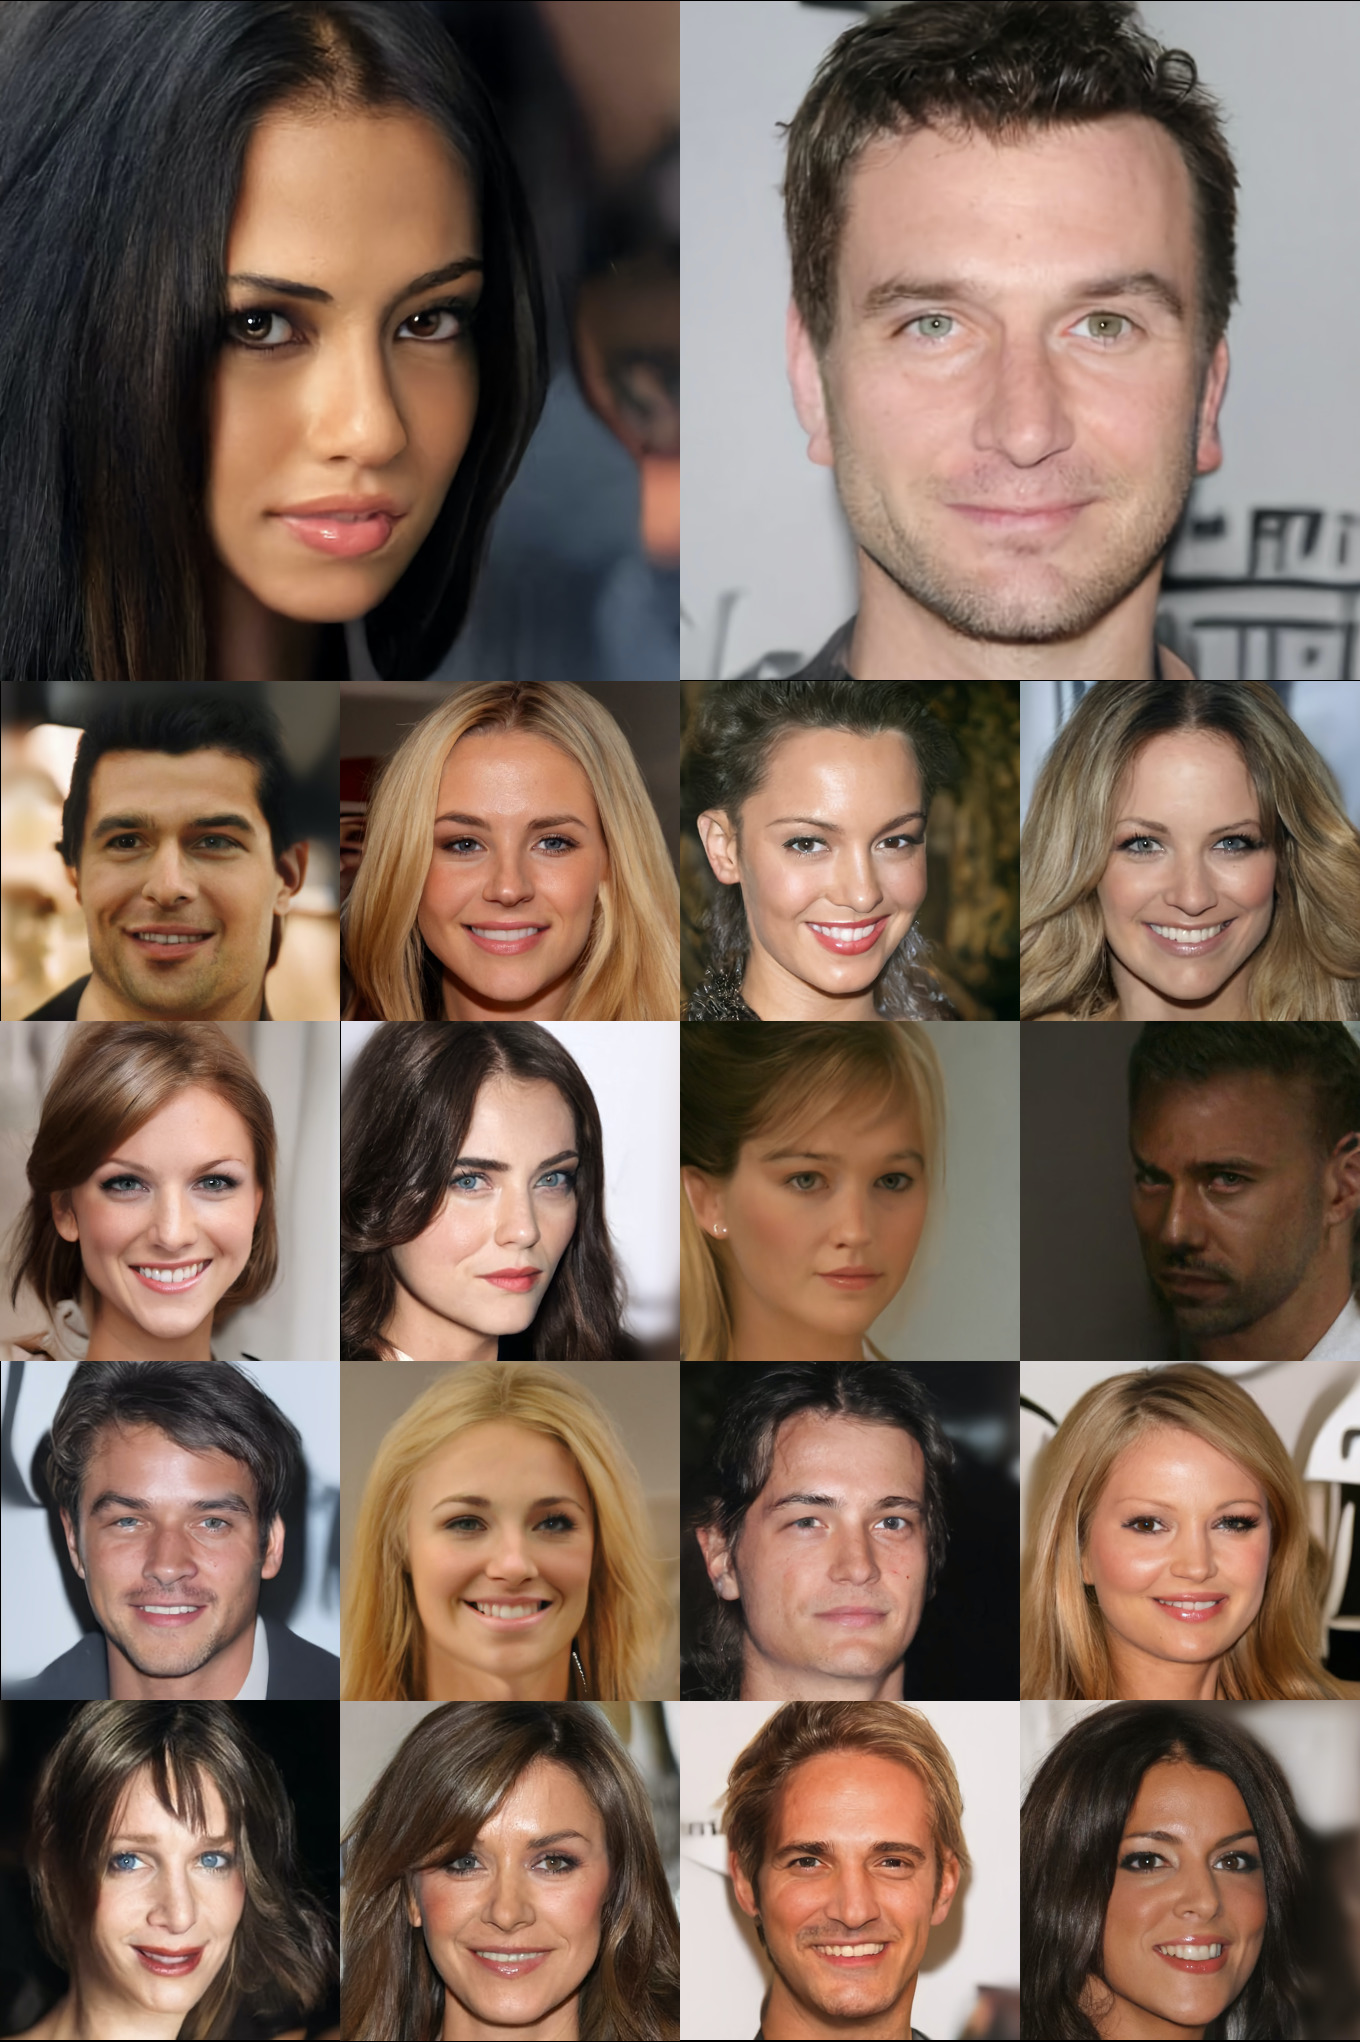
\includegraphics[width=\linewidth]{figures/combine.jpg}
    \caption{Samples on $1024\times 1024$ CelebA-HQ from continuously trained NCSN++.}
    \label{fig:celebahq}
\end{figure}


\subsection{High resolution images} 
\label{app:hq}

Encouraged by the success of NCSN++ on CIFAR-10, we proceed to test it on $1024\times 1024$ CelebA-HQ~\citep{karras2018progressive}, a task that was previously only achievable by some GAN models and VQ-VAE-2~\citep{razavi2019generating}. We used a batch size of 8, increased the EMA rate to 0.9999, and trained the NCSN++ model with the continuous objective (\cref{eqn:training}) for around 700k iterations. We use the PC sampler discretized at 2000 steps with one Langevin step per noise scale and a signal-to-noise ratio of 0.15. The scale parameter for the random Fourier feature embeddings is fixed to 4. We use the ``residual'' progressive architecture for the input, and ``output\_skip'' progressive architecture for the output. We provide samples in \cref{fig:celebahq}. Although these samples are not perfect (\eg, there are visible flaws on facial symmetry), we believe these results are encouraging and can demonstrate the scalability of our approach. Future work on more effective architectures are likely to significantly advance the performance of score-based generative models on this task.


\section{Controllable generation}\label{app:cond_gen}
Consider a forward SDE with the following general form
\begin{align*}
     \ud \bfx = \bff(\bfx, t) \ud t + \mbf{G}(\bfx, t) \ud \bfw,
\end{align*}
and suppose the initial state distribution is $p_0(\bfx(0) \mid \bfy)$. The density at time $t$ is $p_t(\bfx(t) \mid \bfy)$ when conditioned on $\bfy$. Therefore, using \citet{Anderson1982-ny}, the reverse-time SDE is given by
\begin{align}
\resizebox{0.92\linewidth}{!}{$\displaystyle \ud \bfx = \{\bff(\bfx, t) - \nabla \cdot [\bfG(\bfx, t) \bfG(\bfx,t)\tran] - \bfG(\bfx,t)\bfG(\bfx,t)\tran  \nabla_\bfx  \log p_t(\bfx \mid \bfy)\} \ud t + \mbf{G}(\bfx, t) \ud \bar{\bfw}$} \label{eqn:cond_sde_2}.
\end{align}
Since $p_t(\bfx(t) \mid \bfy) \propto p_t(\bfx(t)) p(\bfy \mid \bfx(t))$, the score $\nabla_\bfx \log p_t(\bfx(t) \mid \bfy)$ can be computed easily by
\begin{align}
    \nabla_{\bfx} \log p_t(\bfx(t) \mid \bfy) = \nabla_{\bfx} \log p_t(\bfx(t)) + \nabla_{\bfx} \log p(\bfy \mid \bfx(t)).
\end{align}
This subsumes the conditional reverse-time SDE in \cref{eqn:cond_sde} as a special case. All sampling methods we have discussed so far can be applied to the conditional reverse-time SDE for sample generation.

\subsection{Class-conditional sampling}\label{app:class_cond_sampling}
When $\bfy$ represents class labels, we can train a time-dependent classifier $p_t(\bfy \mid \bfx(t))$ for class-conditional sampling. Since the forward SDE is tractable, we can easily create a pair of training data $(\bfx(t), \bfy)$ by first sampling $(\bfx(0), \bfy)$ from a dataset and then obtaining $\bfx(t) \sim p_{0t}(\bfx(t) \mid \bfx(0))$. Afterwards, we may employ a mixture of cross-entropy losses over different time steps, like \cref{eqn:training}, to train the time-dependent classifier $p_t(\bfy \mid \bfx(t))$.

To test this idea, we trained a Wide ResNet~\citep{zagoruyko2016wide} (\verb|Wide-ResNet-28-10|) on CIFAR-10 with VE perturbations. The classifier is conditioned on $\log \sigma_i$ using random Fourier features~\citep{tancik2020fourfeat}, and the training objective is a simple sum of cross-entropy losses sampled at different scales. We provide a plot to show the accuracy of this classifier over noise scales in \cref{fig:cond_sample_extend}. The score-based model is an unconditional NCSN++ (4 blocks/resolution) in \cref{tab:fid}, and we generate samples using the PC algorithm with 2000 discretization steps. The class-conditional samples are provided in \cref{fig:cond_gen}, and an extended set of conditional samples is given in \cref{fig:cond_sample_extend}.
\begin{figure}
    \centering
    \begin{subfigure}{0.32\textwidth}
        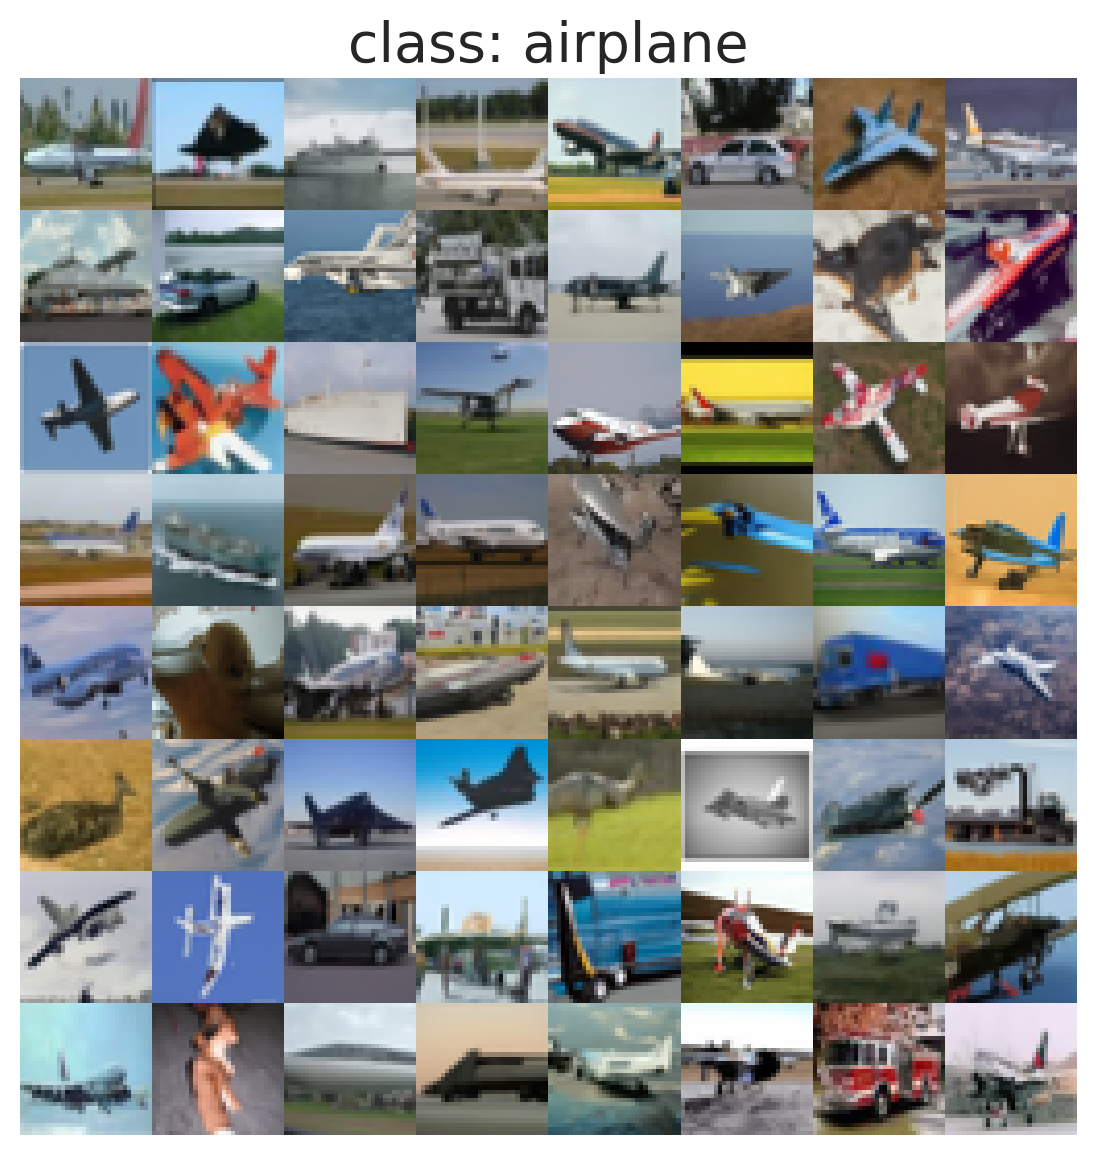
\includegraphics[width=\textwidth]{figures/conditional_shallow_0.png}
    \end{subfigure}
    \begin{subfigure}{0.32\textwidth}
        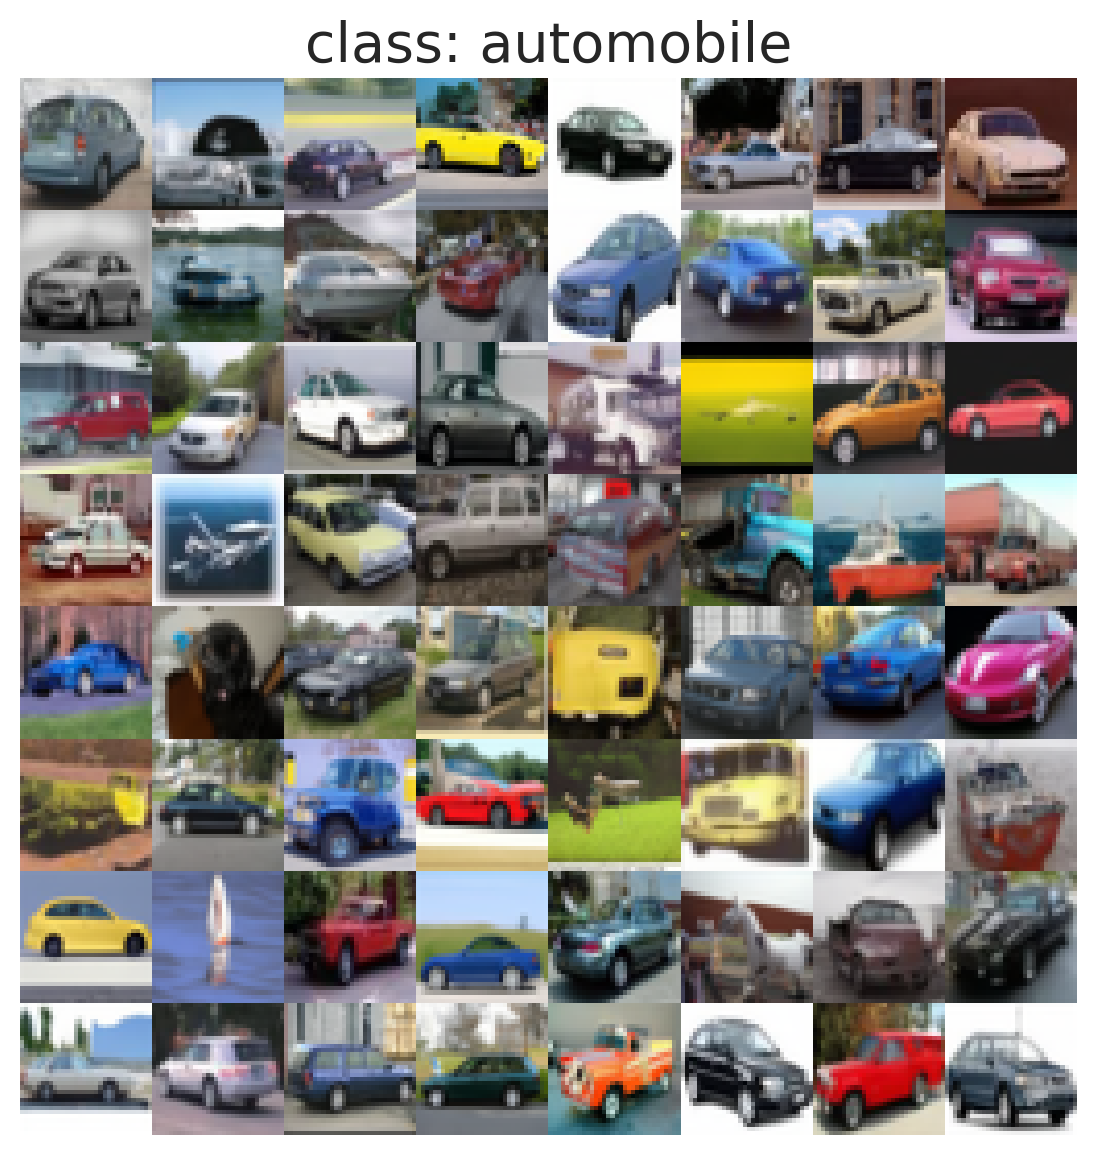
\includegraphics[width=\textwidth]{figures/conditional_shallow_1.png}
    \end{subfigure}
    \begin{subfigure}{0.32\textwidth}
        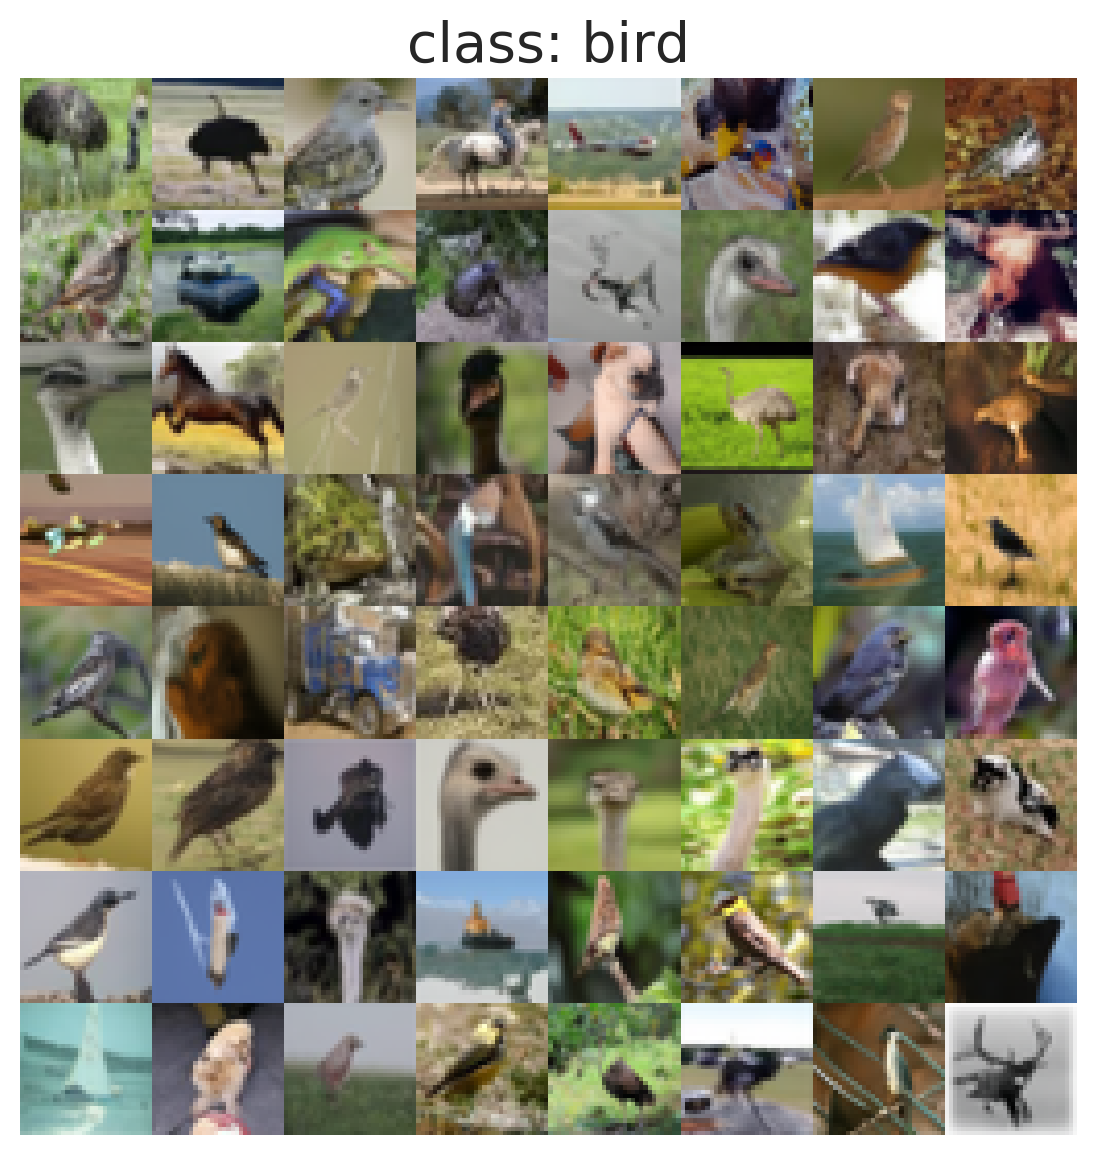
\includegraphics[width=\textwidth]{figures/conditional_shallow_2.png}
    \end{subfigure}\\
    \begin{subfigure}{0.32\textwidth}
        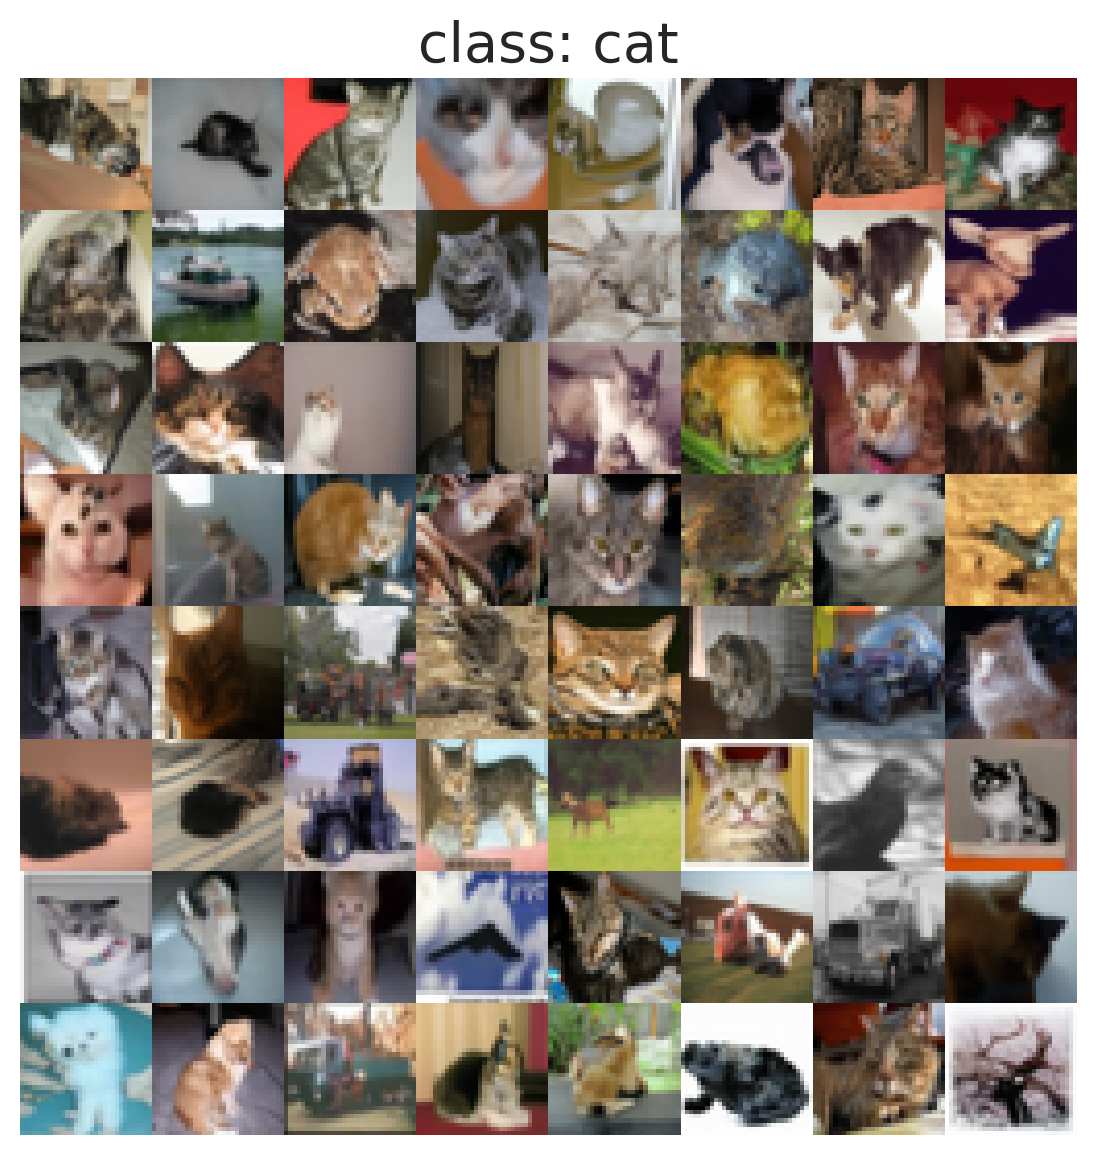
\includegraphics[width=\textwidth]{figures/conditional_shallow_3.png}
    \end{subfigure}
    \begin{subfigure}{0.32\textwidth}
        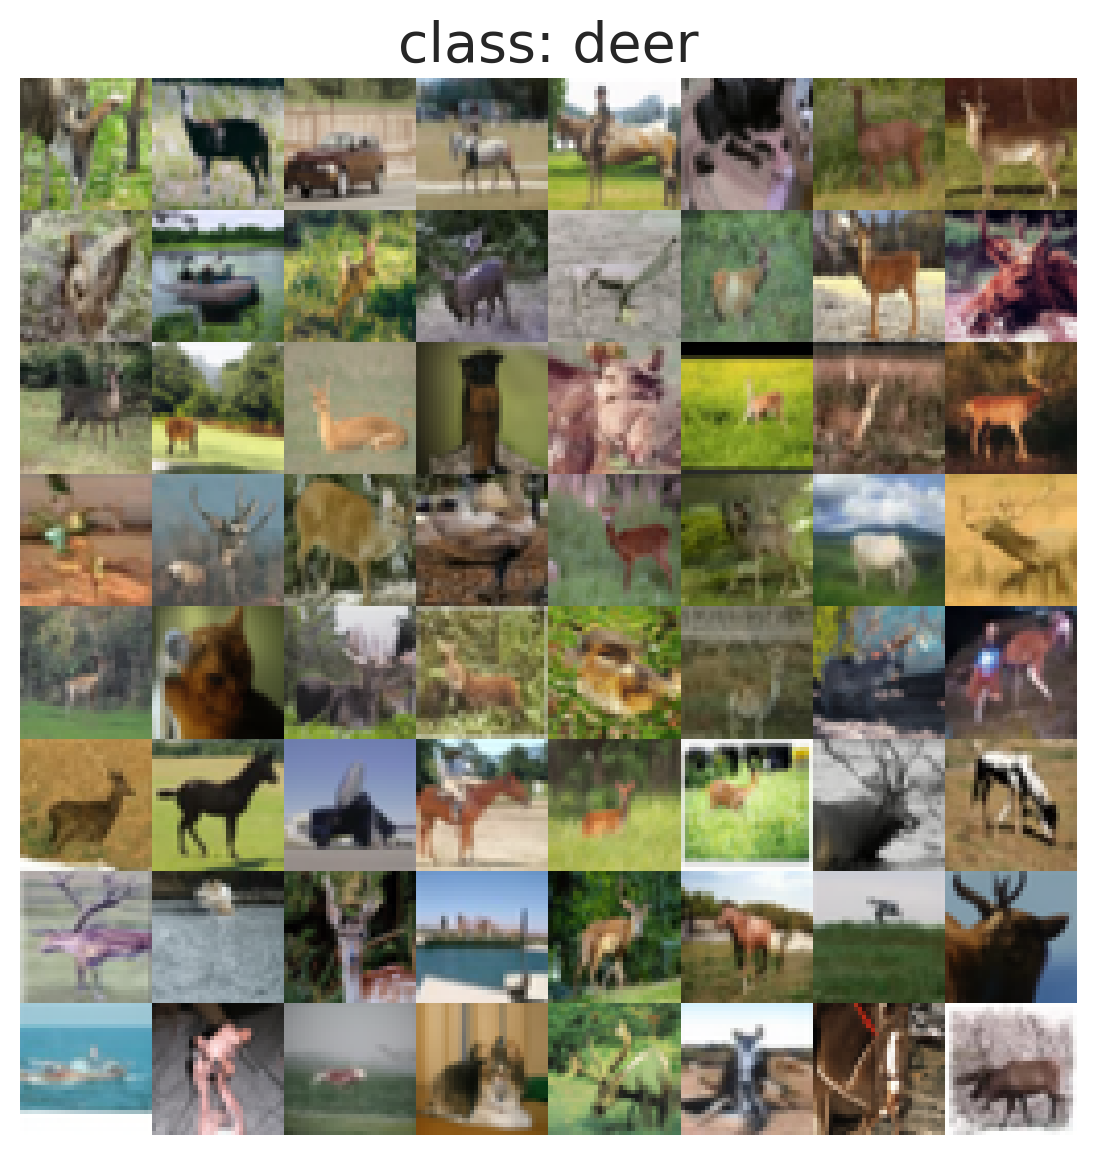
\includegraphics[width=\textwidth]{figures/conditional_shallow_4.png}
    \end{subfigure}
    \begin{subfigure}{0.32\textwidth}
        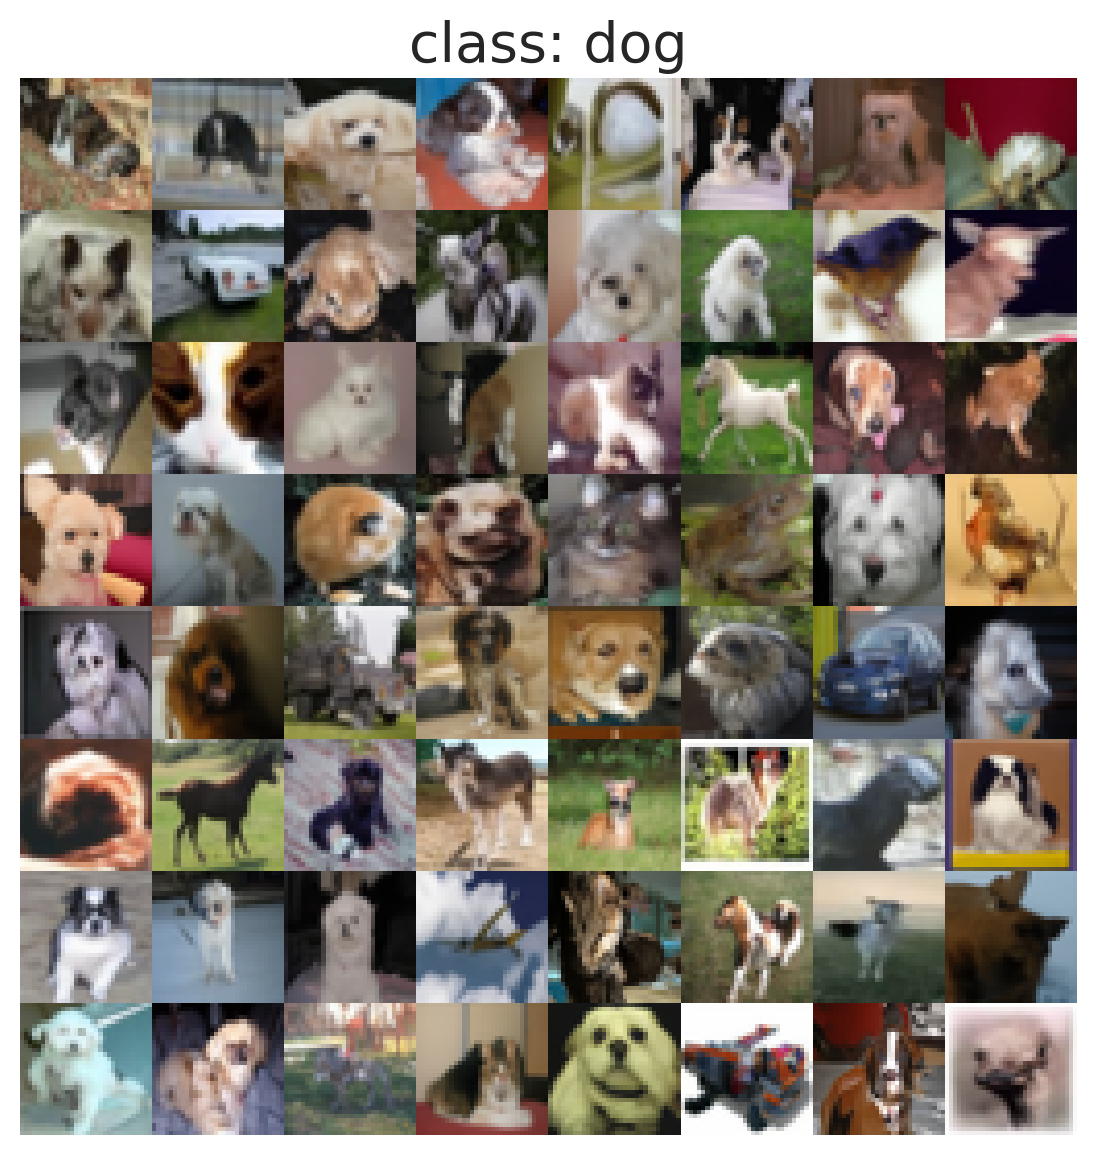
\includegraphics[width=\textwidth]{figures/conditional_shallow_5.png}
    \end{subfigure}\\
    \begin{subfigure}{0.32\textwidth}
        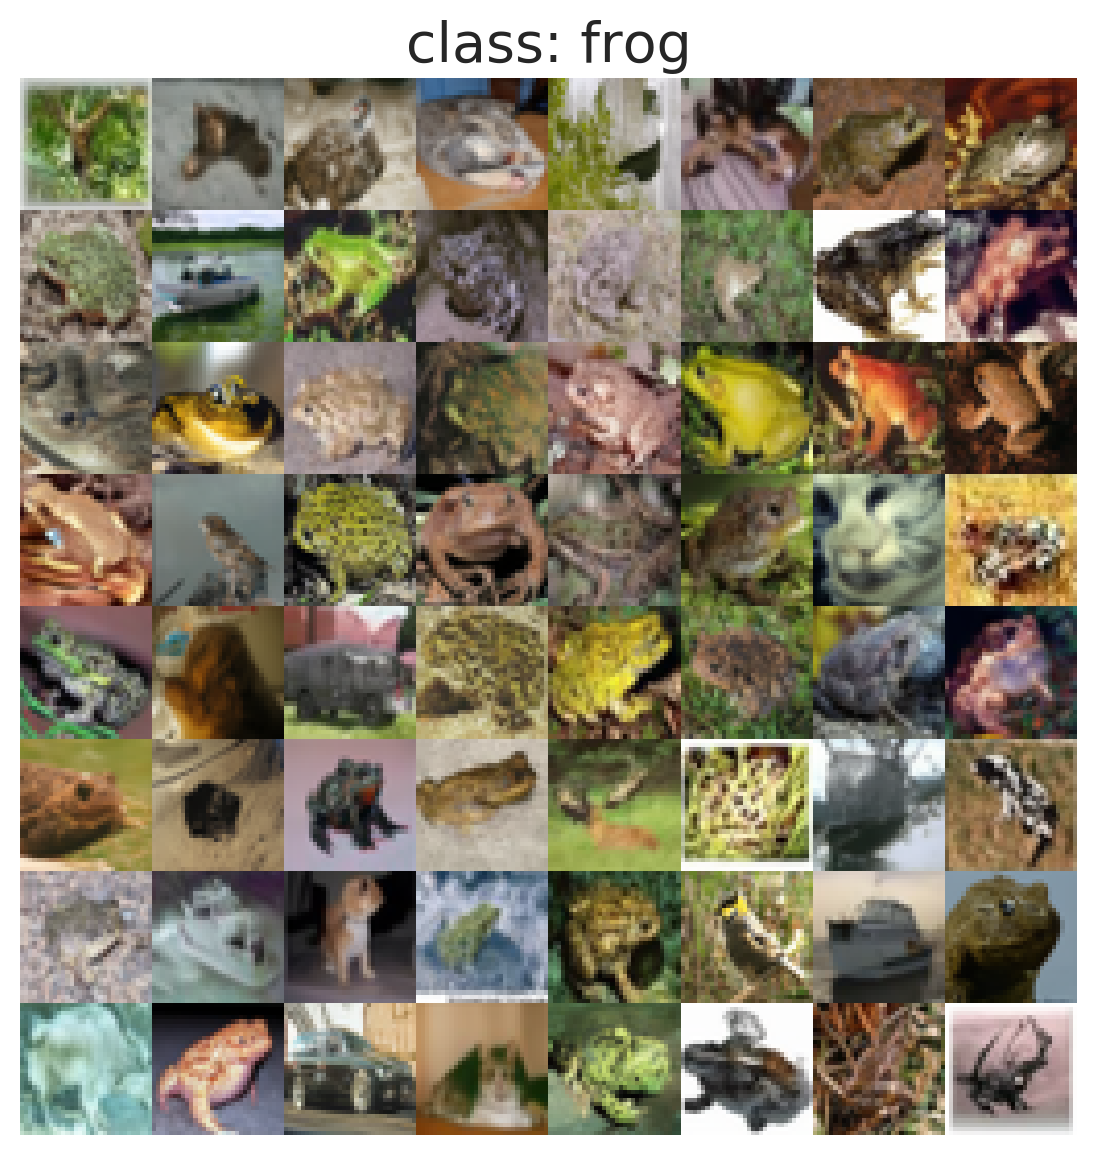
\includegraphics[width=\textwidth]{figures/conditional_shallow_6.png}
    \end{subfigure}
    \begin{subfigure}{0.32\textwidth}
        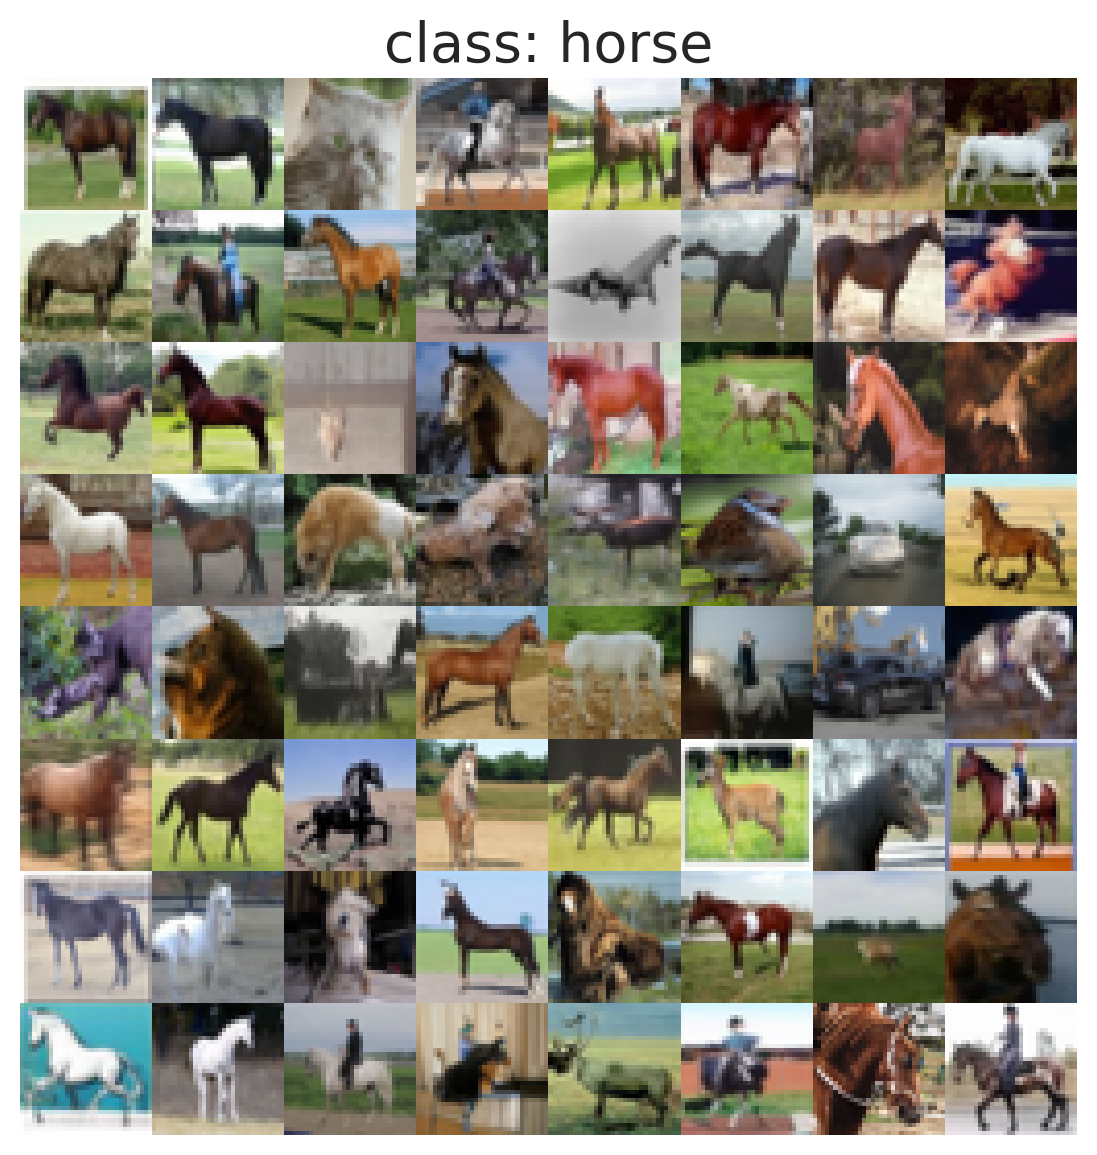
\includegraphics[width=\textwidth]{figures/conditional_shallow_7.png}
    \end{subfigure}
    \begin{subfigure}{0.32\textwidth}
        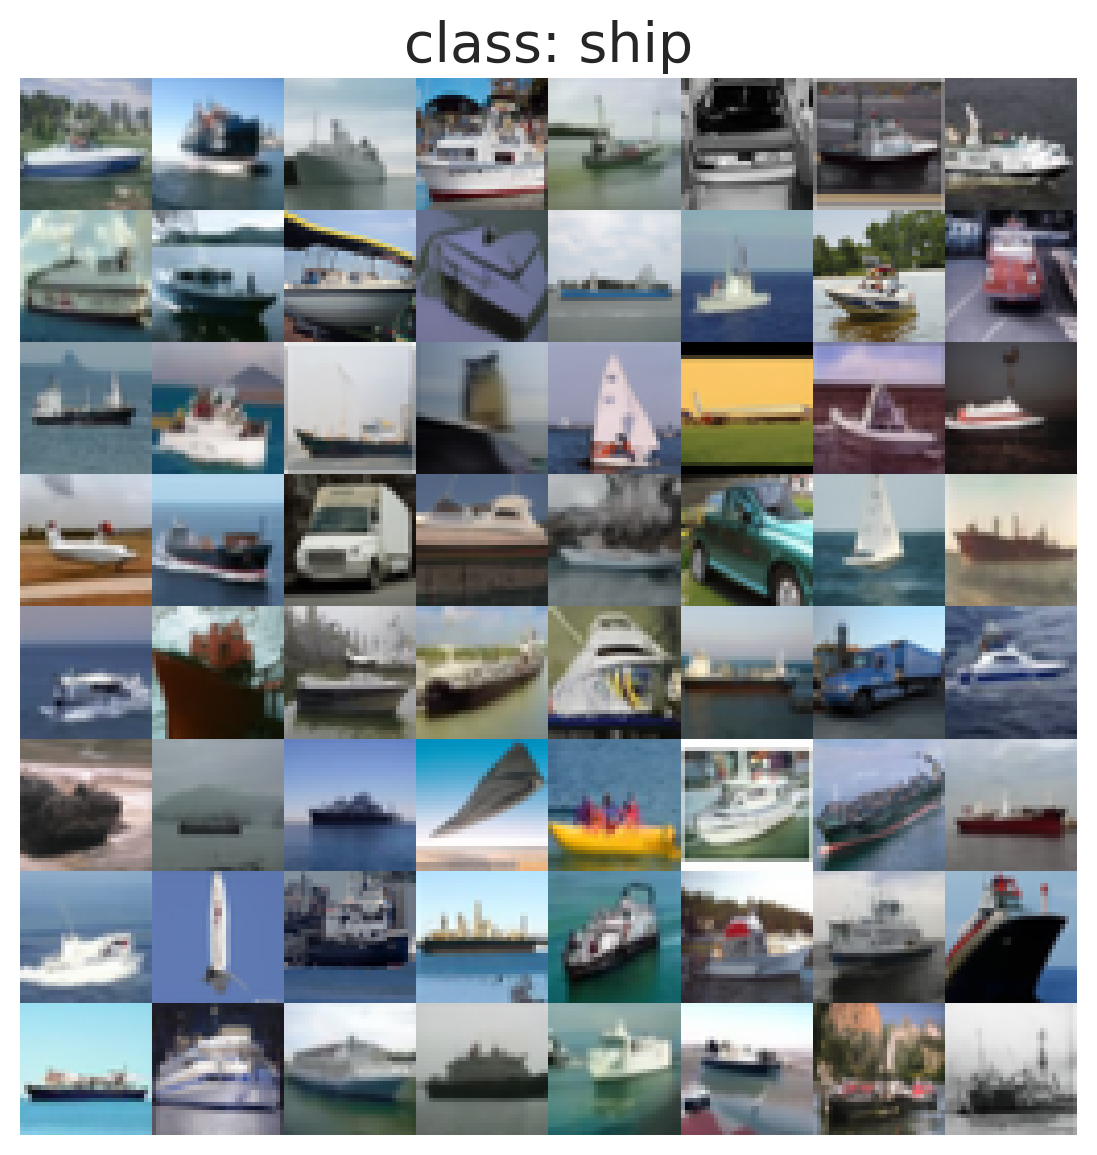
\includegraphics[width=\textwidth]{figures/conditional_shallow_8.png}
    \end{subfigure}\\
    \begin{subfigure}{0.32\textwidth}
        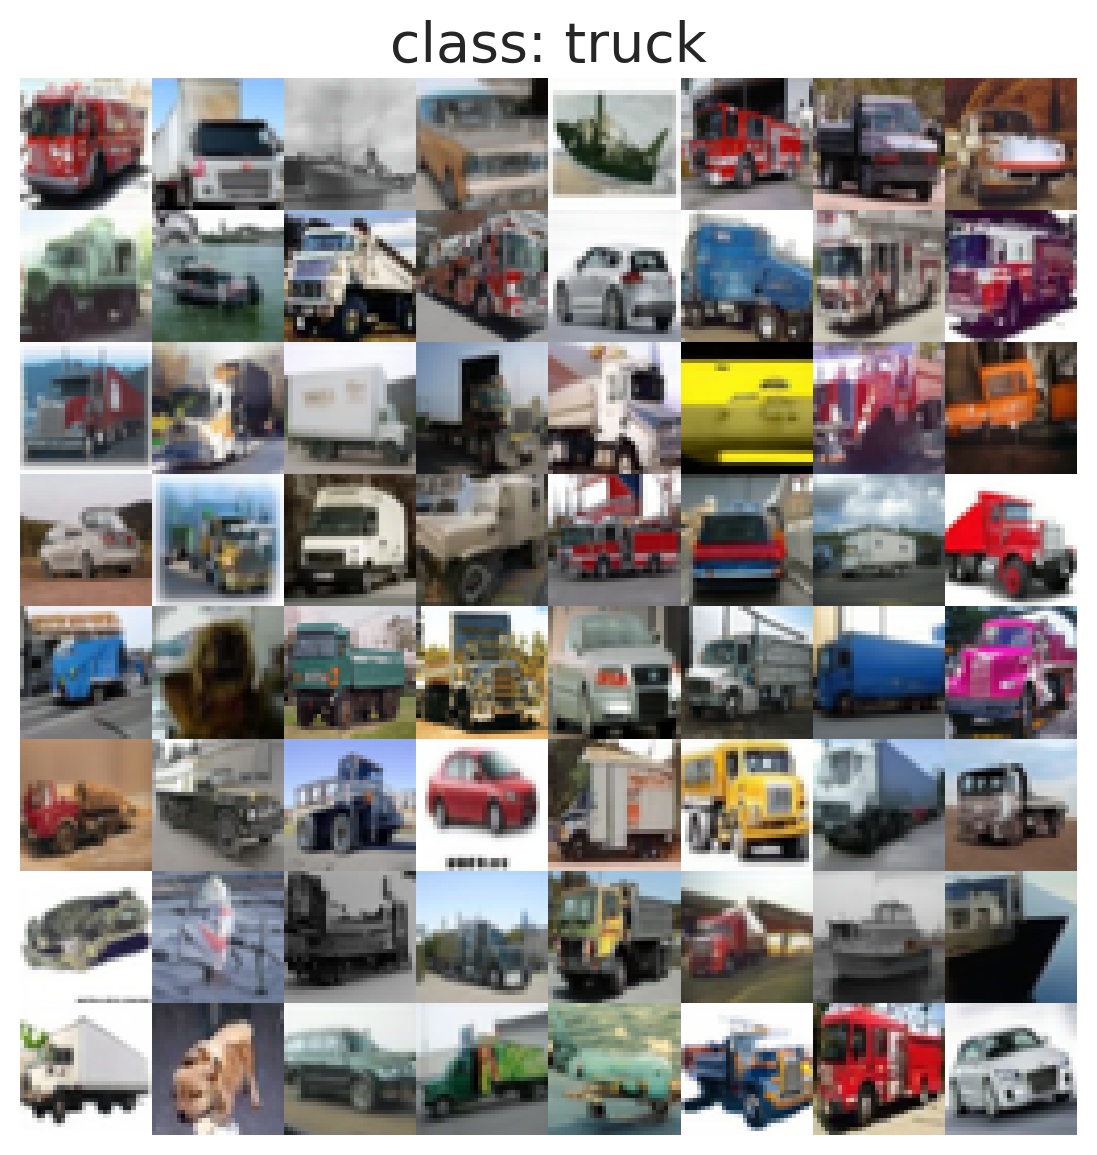
\includegraphics[width=\textwidth]{figures/conditional_shallow_9.png}
    \end{subfigure}
    \begin{subfigure}{0.4\textwidth}
        \includegraphics[width=\textwidth]{figures/accuracy_curve.pdf}
    \end{subfigure}
    \caption{Class-conditional image generation by solving the conditional reverse-time SDE with PC. The curve shows the accuracy of our noise-conditional classifier over different noise scales.}
    \label{fig:cond_sample_extend}
\end{figure}

\subsection{Imputation} \label{app:imputation}
Imputation is a special case of conditional sampling. Denote by $\Omega(\bfx)$ and $\bomega(\bfx)$ the known and unknown dimensions of $\bfx$ respectively, and let $\bff_{\bomega}(\cdot, t)$ and $\bfG_{\bomega}(\cdot, t)$ denote $\bff(\cdot, t)$ and $\bfG(\cdot, t)$ restricted to the unknown dimensions. For VE/VP SDEs, the drift coefficient $\bff(\cdot, t)$ is element-wise, and the diffusion coefficient $\bfG(\cdot, t)$ is diagonal. When $\bff(\cdot, t)$ is element-wise, $\bff_{\bomega}(\cdot, t)$ denotes the same element-wise function applied only to the unknown dimensions. When $\bfG(\cdot, t)$ is diagonal, $\bfG_{\bomega}(\cdot, t)$ denotes the sub-matrix restricted to unknown dimensions. 

For imputation, our goal is to sample from $p(\bomega(\bfx(0)) \mid \Omega(\bfx(0)) = \bfy)$. Define a new diffusion process $\bfz(t) = \bomega(\bfx(t))$, and note that the SDE for $\bfz(t)$ can be written as
\begin{align*}
\ud \bfz = \bff_\bomega(\bfz, t) \ud t + \bfG_\bomega(\bfz, t) \ud \bfw.
\end{align*}
The reverse-time SDE, conditioned on $\Omega(\bfx(0)) = \bfy$, is given by
\begin{multline*}
\ud\bfz = \big\{\bff_\bomega(\bfz, t) - \nabla \cdot [\bfG_{\bomega}(\bfz, t) \bfG_{\bomega}(\bfz,t)\tran] \\- \bfG_\bomega(\bfz, t)\bfG_\bomega(\bfz, t)\tran \nabla_\bfz \log p_t(\bfz \mid \Omega(\bfz(0)) = \bfy)\big\}\ud t + \bfG_\bomega(\bfz, t)\ud\bar{\bfw}.
\end{multline*}
Although $p_t(\bfz(t) \mid \Omega(\bfx(0)) = \bfy)$ is in general intractable, it can be approximated. Let $A$ denote the event $\Omega(\bfx(0)) = \bfy $. We have
\begin{align*}
p_t(\bfz(t) \mid \Omega(\bfx(0)) = \bfy) = p_t(\bfz(t) \mid A) &= \int p_t(\bfz(t) \mid \Omega(\bfx(t)), A) p_t(\Omega(\bfx(t)) \mid A) \ud \Omega(\bfx(t)) \\
&= \mathbb{E}_{p_t(\Omega(\bfx(t)) \mid A)}[p_t(\bfz(t) \mid \Omega(\bfx(t)), A)]\\
&\approx \mathbb{E}_{p_t(\Omega(\bfx(t)) \mid A)}[p_t(\bfz(t) \mid \Omega(\bfx(t)))]\\
&\approx p_t(\bfz(t) \mid \hat{\Omega}(\bfx(t))),
\end{align*}
where $\hat{\Omega}(\bfx(t))$ is a random sample from $p_t(\Omega(\bfx(t)) \mid A)$, which is typically a tractable distribution. Therefore,
\begin{align*}
\nabla_\bfz \log p_t(\bfz(t) \mid \Omega(\bfx(0))=\bfy) &\approx \nabla_\bfz \log p_t(\bfz(t) \mid \hat{\Omega}(\bfx(t))) \\
&= \nabla_\bfz \log p_t([\bfz(t); \hat{\Omega}(\bfx(t))]),
\end{align*}
where $[\bfz(t); \hat{\Omega}(\bfx(t))]$ denotes a vector $\bfu(t)$ such that $\Omega(\bfu(t)) = \hat{\Omega}(\bfx(t))$ and $\bar{\Omega}(\bfu(t)) = \bfz(t)$, and the identity holds because $\nabla_\bfz \log p_t([\bfz(t); \hat{\Omega}(\bfx(t))]) = \nabla_\bfz \log p_t(\bfz(t) \mid \hat{\Omega}(\bfx(t))) + \nabla_\bfz \log p(\hat{\Omega}(\bfx(t))) = \nabla_\bfz \log p_t(\bfz(t) \mid \hat{\Omega}(\bfx(t)))$.

We provided an extended set of inpainting results in \cref{fig:bedroom_inpainting,fig:church_inpainting}.

\begin{figure}
    \centering
    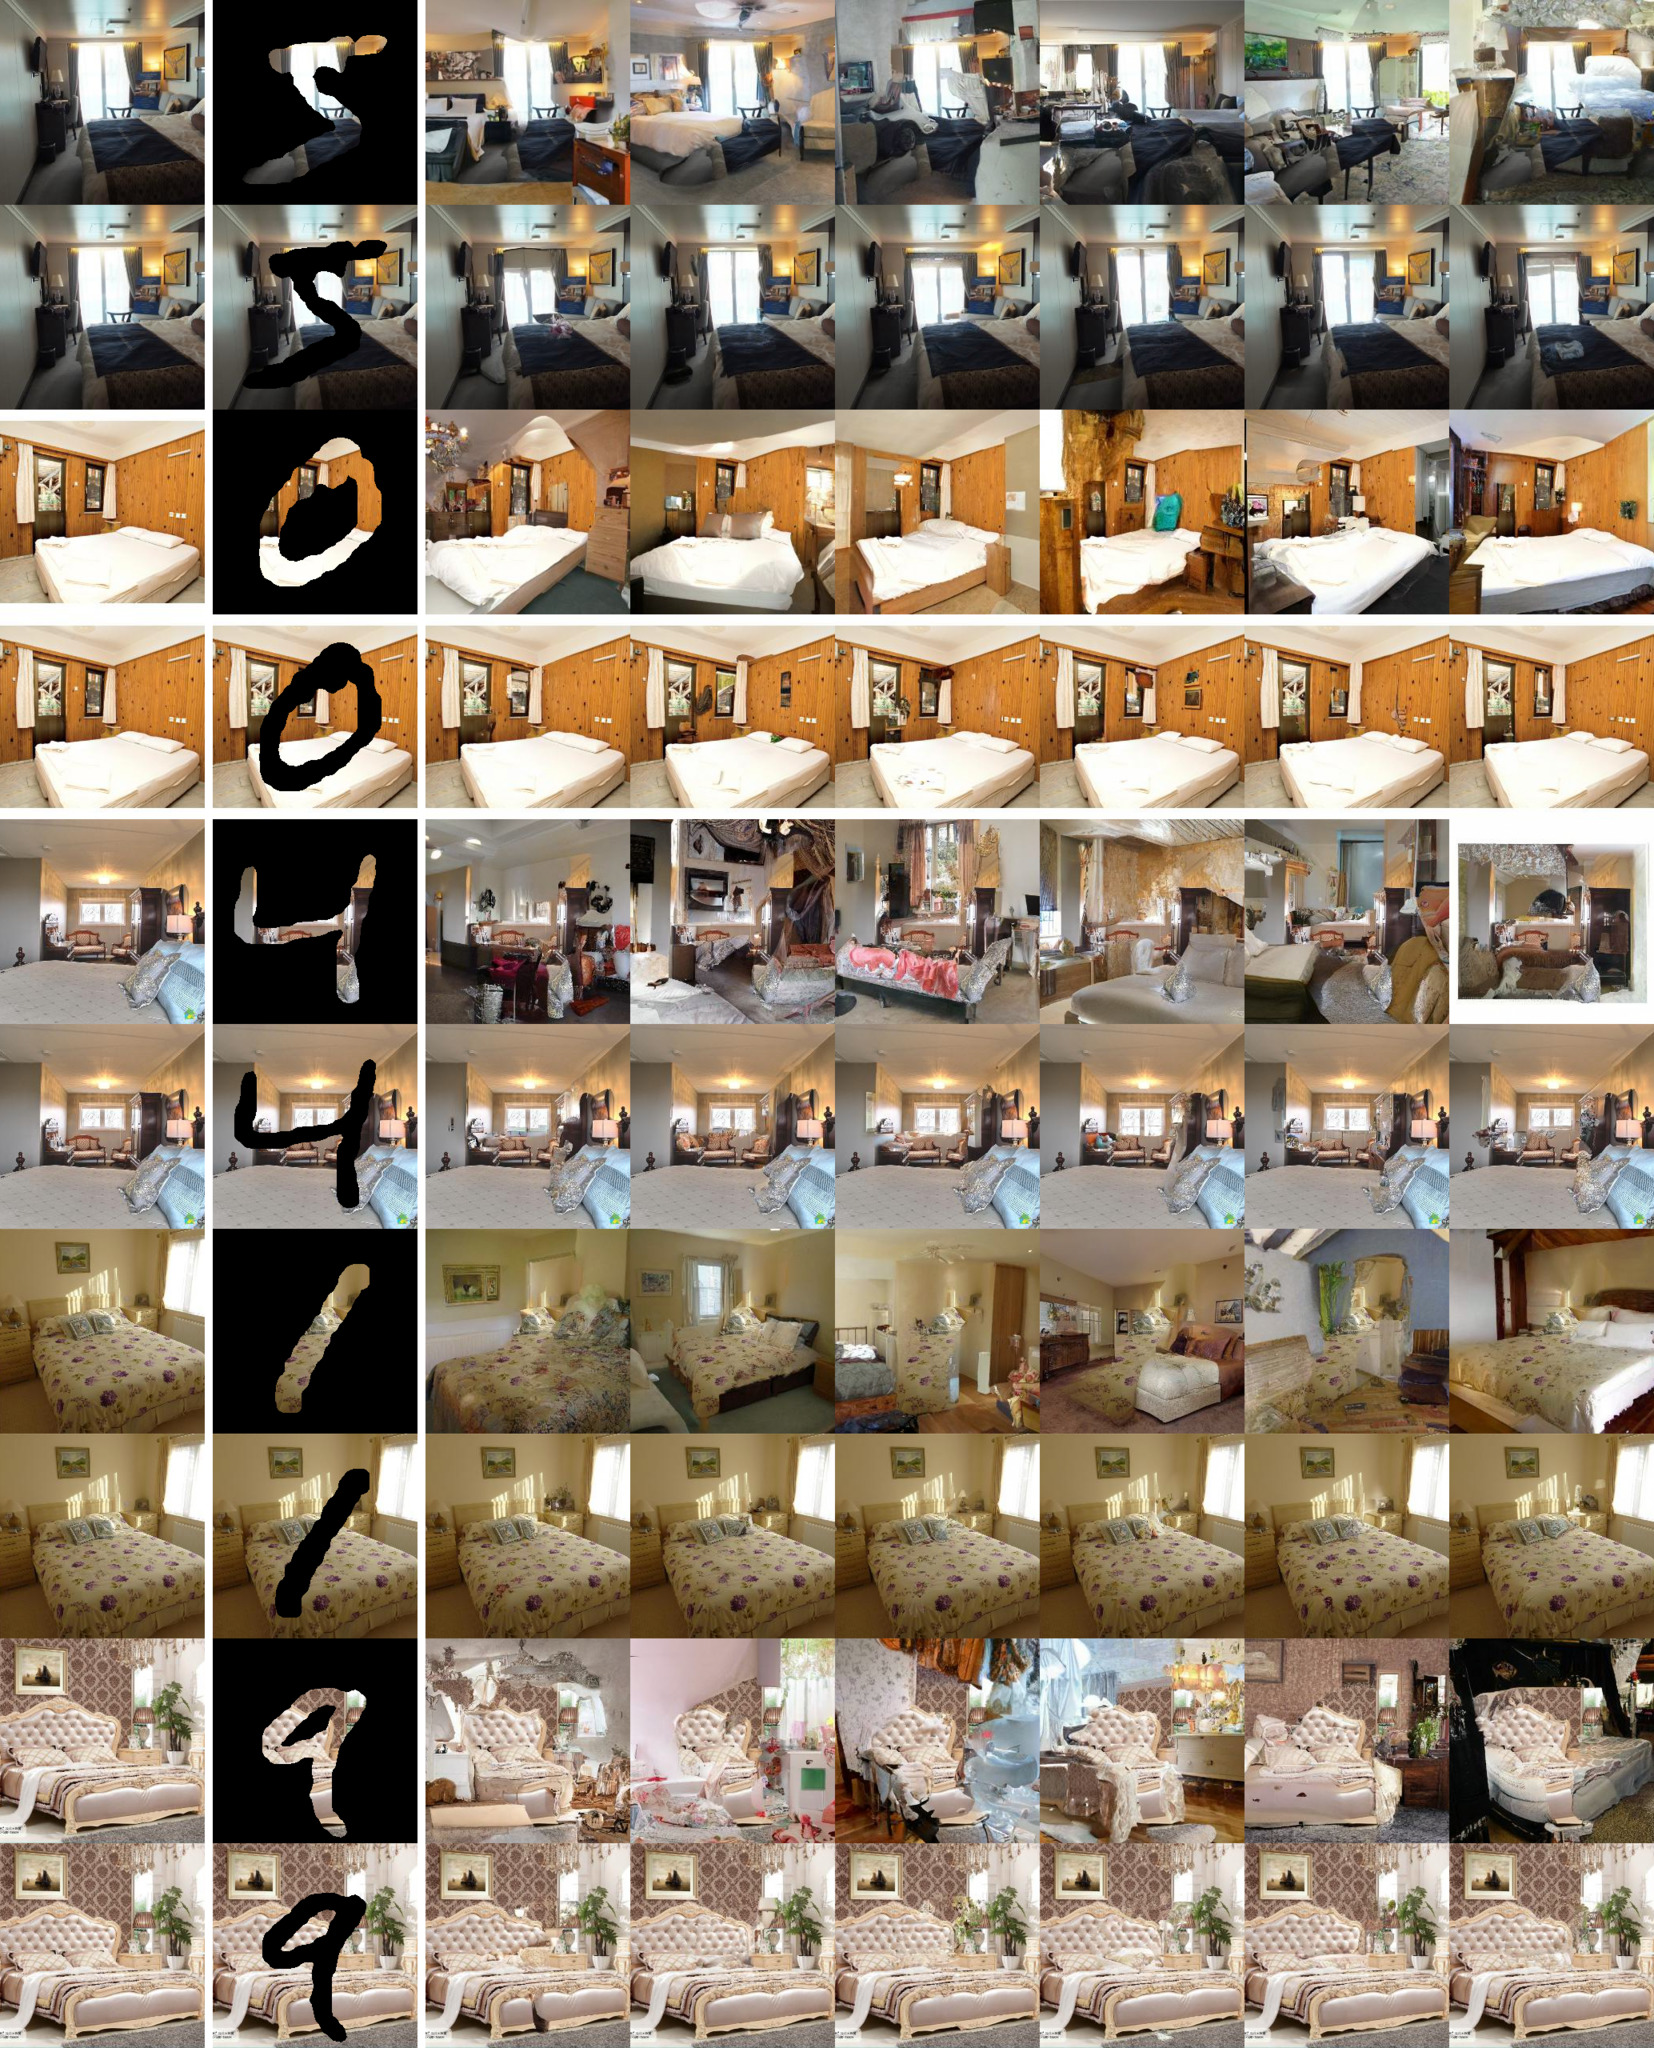
\includegraphics[width=\linewidth]{figures/bedroom_inpainting.jpg}
    \caption{Extended inpainting results for $256\times 256$ bedroom images.}
    \label{fig:bedroom_inpainting}
\end{figure}

\begin{figure}
    \centering
    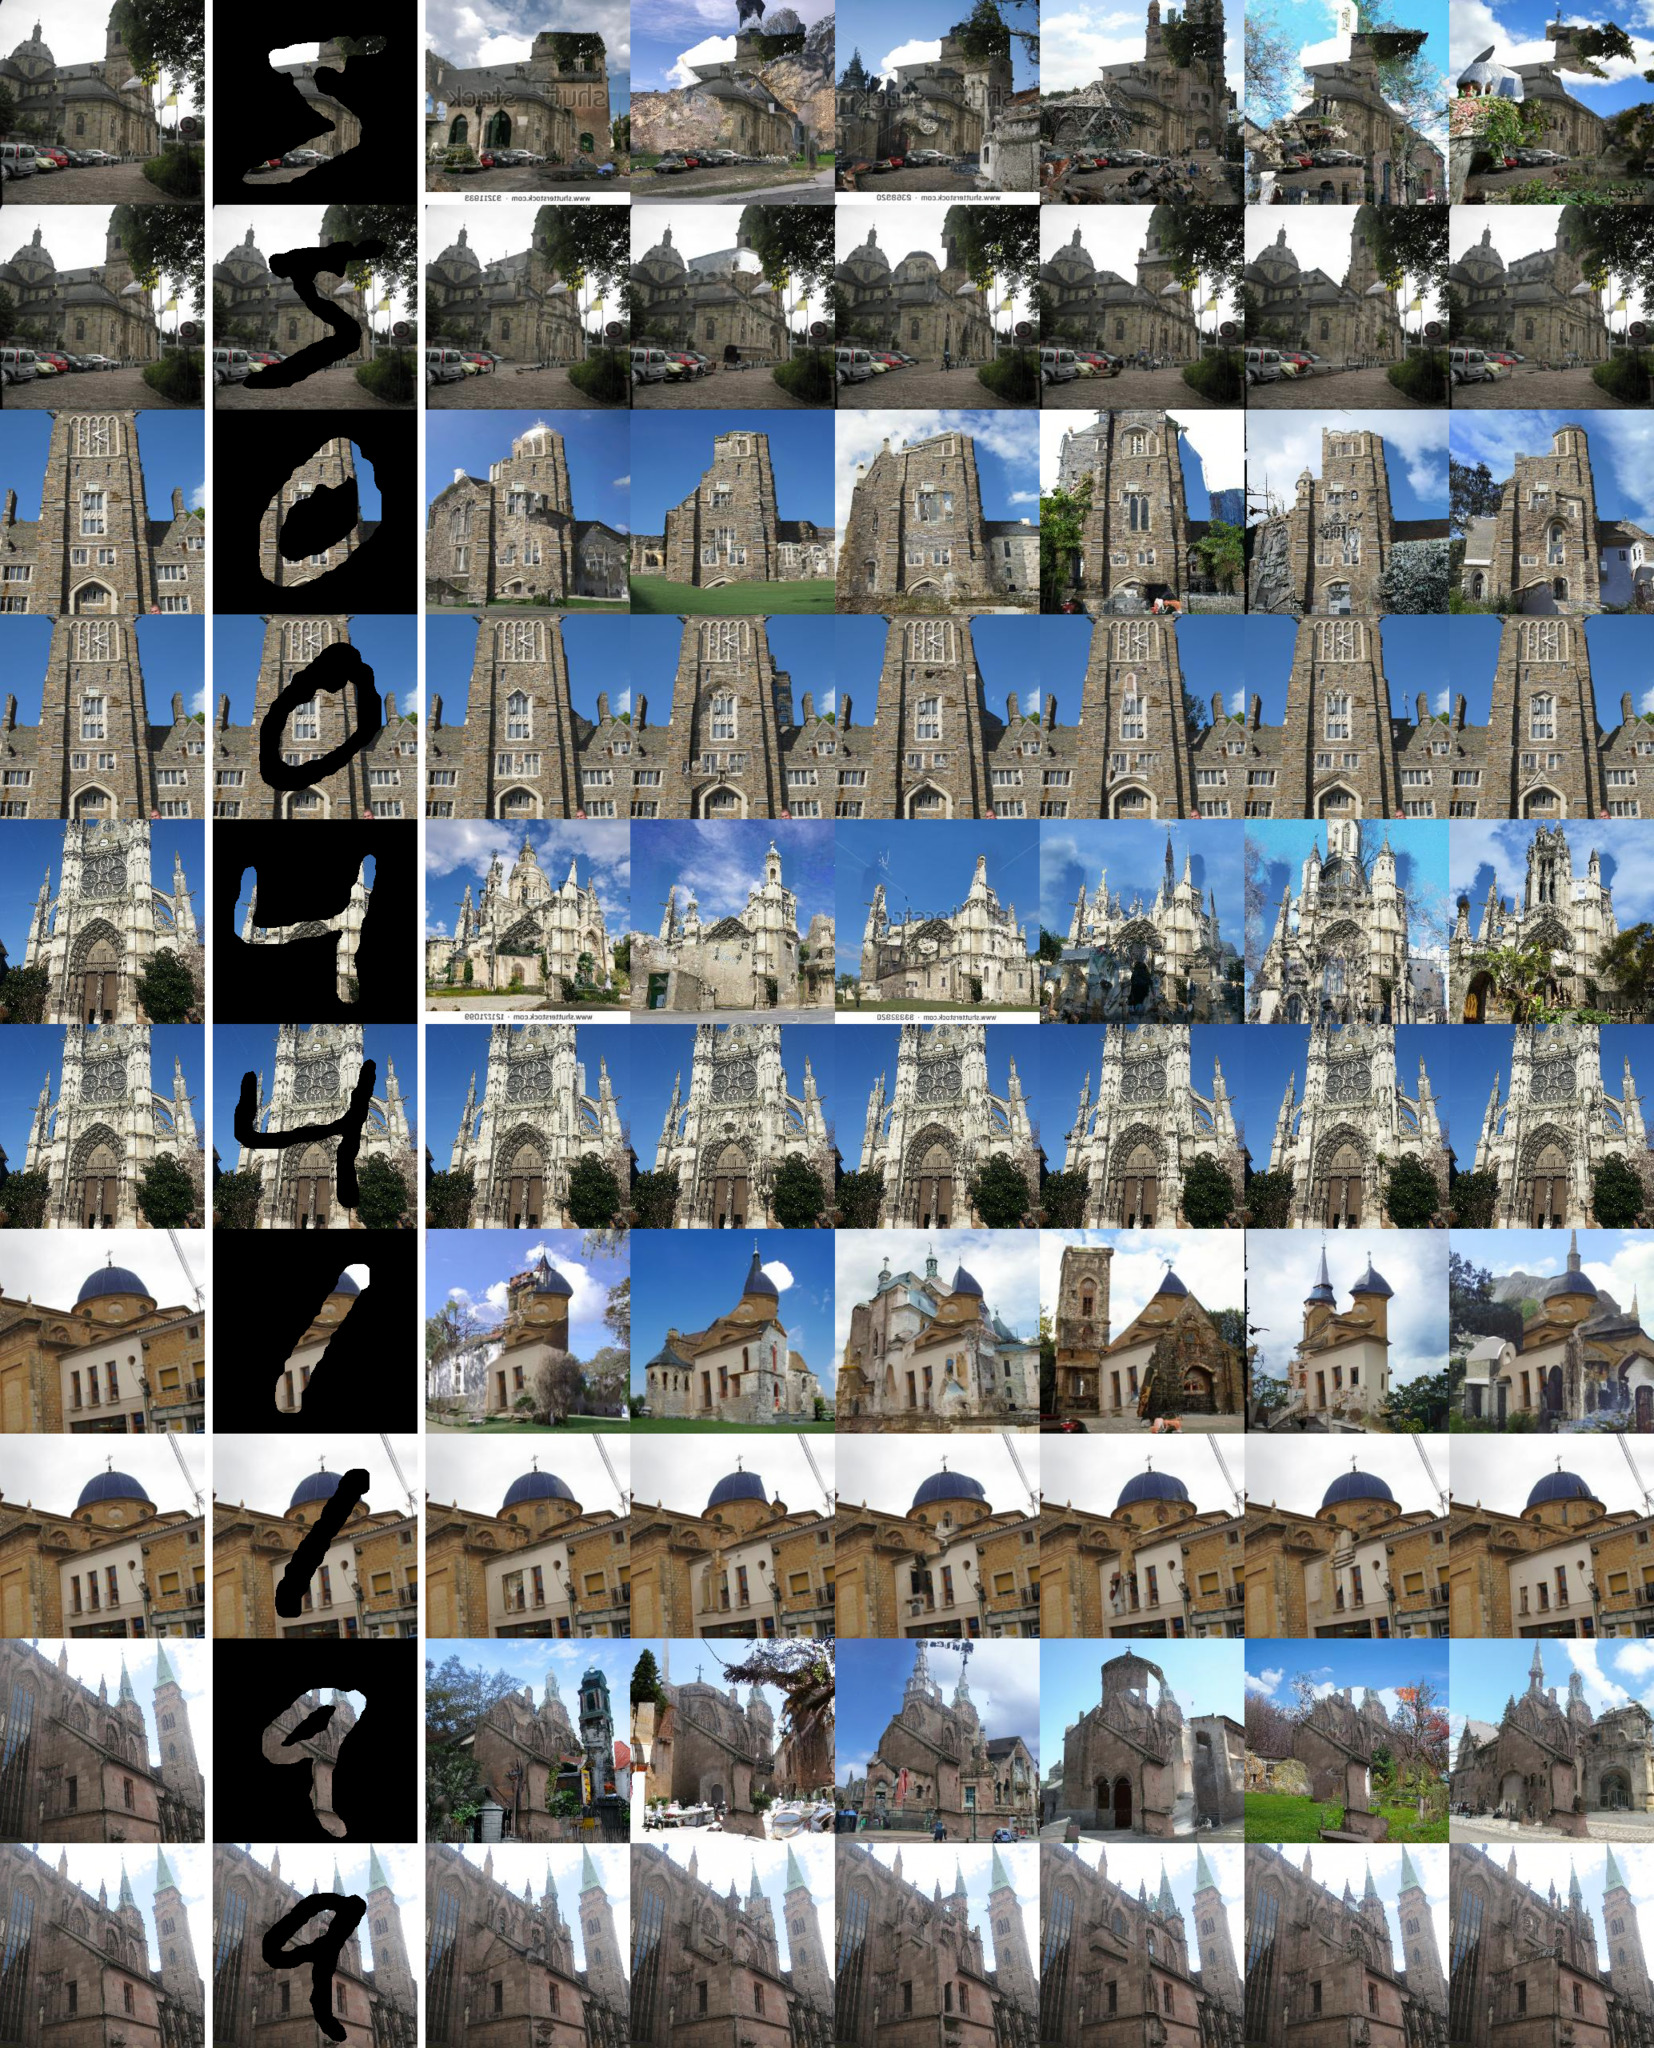
\includegraphics[width=\linewidth]{figures/church_inpainting.jpg}
    \caption{Extended inpainting results for $256\times 256$ church images.}
    \label{fig:church_inpainting}
\end{figure}
\subsection{Colorization}\label{app:colorization}
Colorization is a special case of imputation, except that the known data dimensions are coupled. We can decouple these data dimensions by using an orthogonal linear transformation to map the gray-scale image to a separate channel in a different space, and then perform imputation to complete the other channels before transforming everything back to the original image space. The orthogonal matrix we used to decouple color channels is
\begin{align*}
    \begin{pmatrix}
        0.577 &  -0.816 &  0\\
        0.577 &  0.408 &  0.707\\
        0.577 &  0.408 & -0.707\\
    \end{pmatrix}.
\end{align*}
Because the transformations are all orthogonal matrices, the standard Wiener process $\bfw(t)$ will still be a standard Wiener process in the transformed space, allowing us to build an SDE and use the same imputation method in \cref{app:imputation}.

\begin{figure}
    \centering
    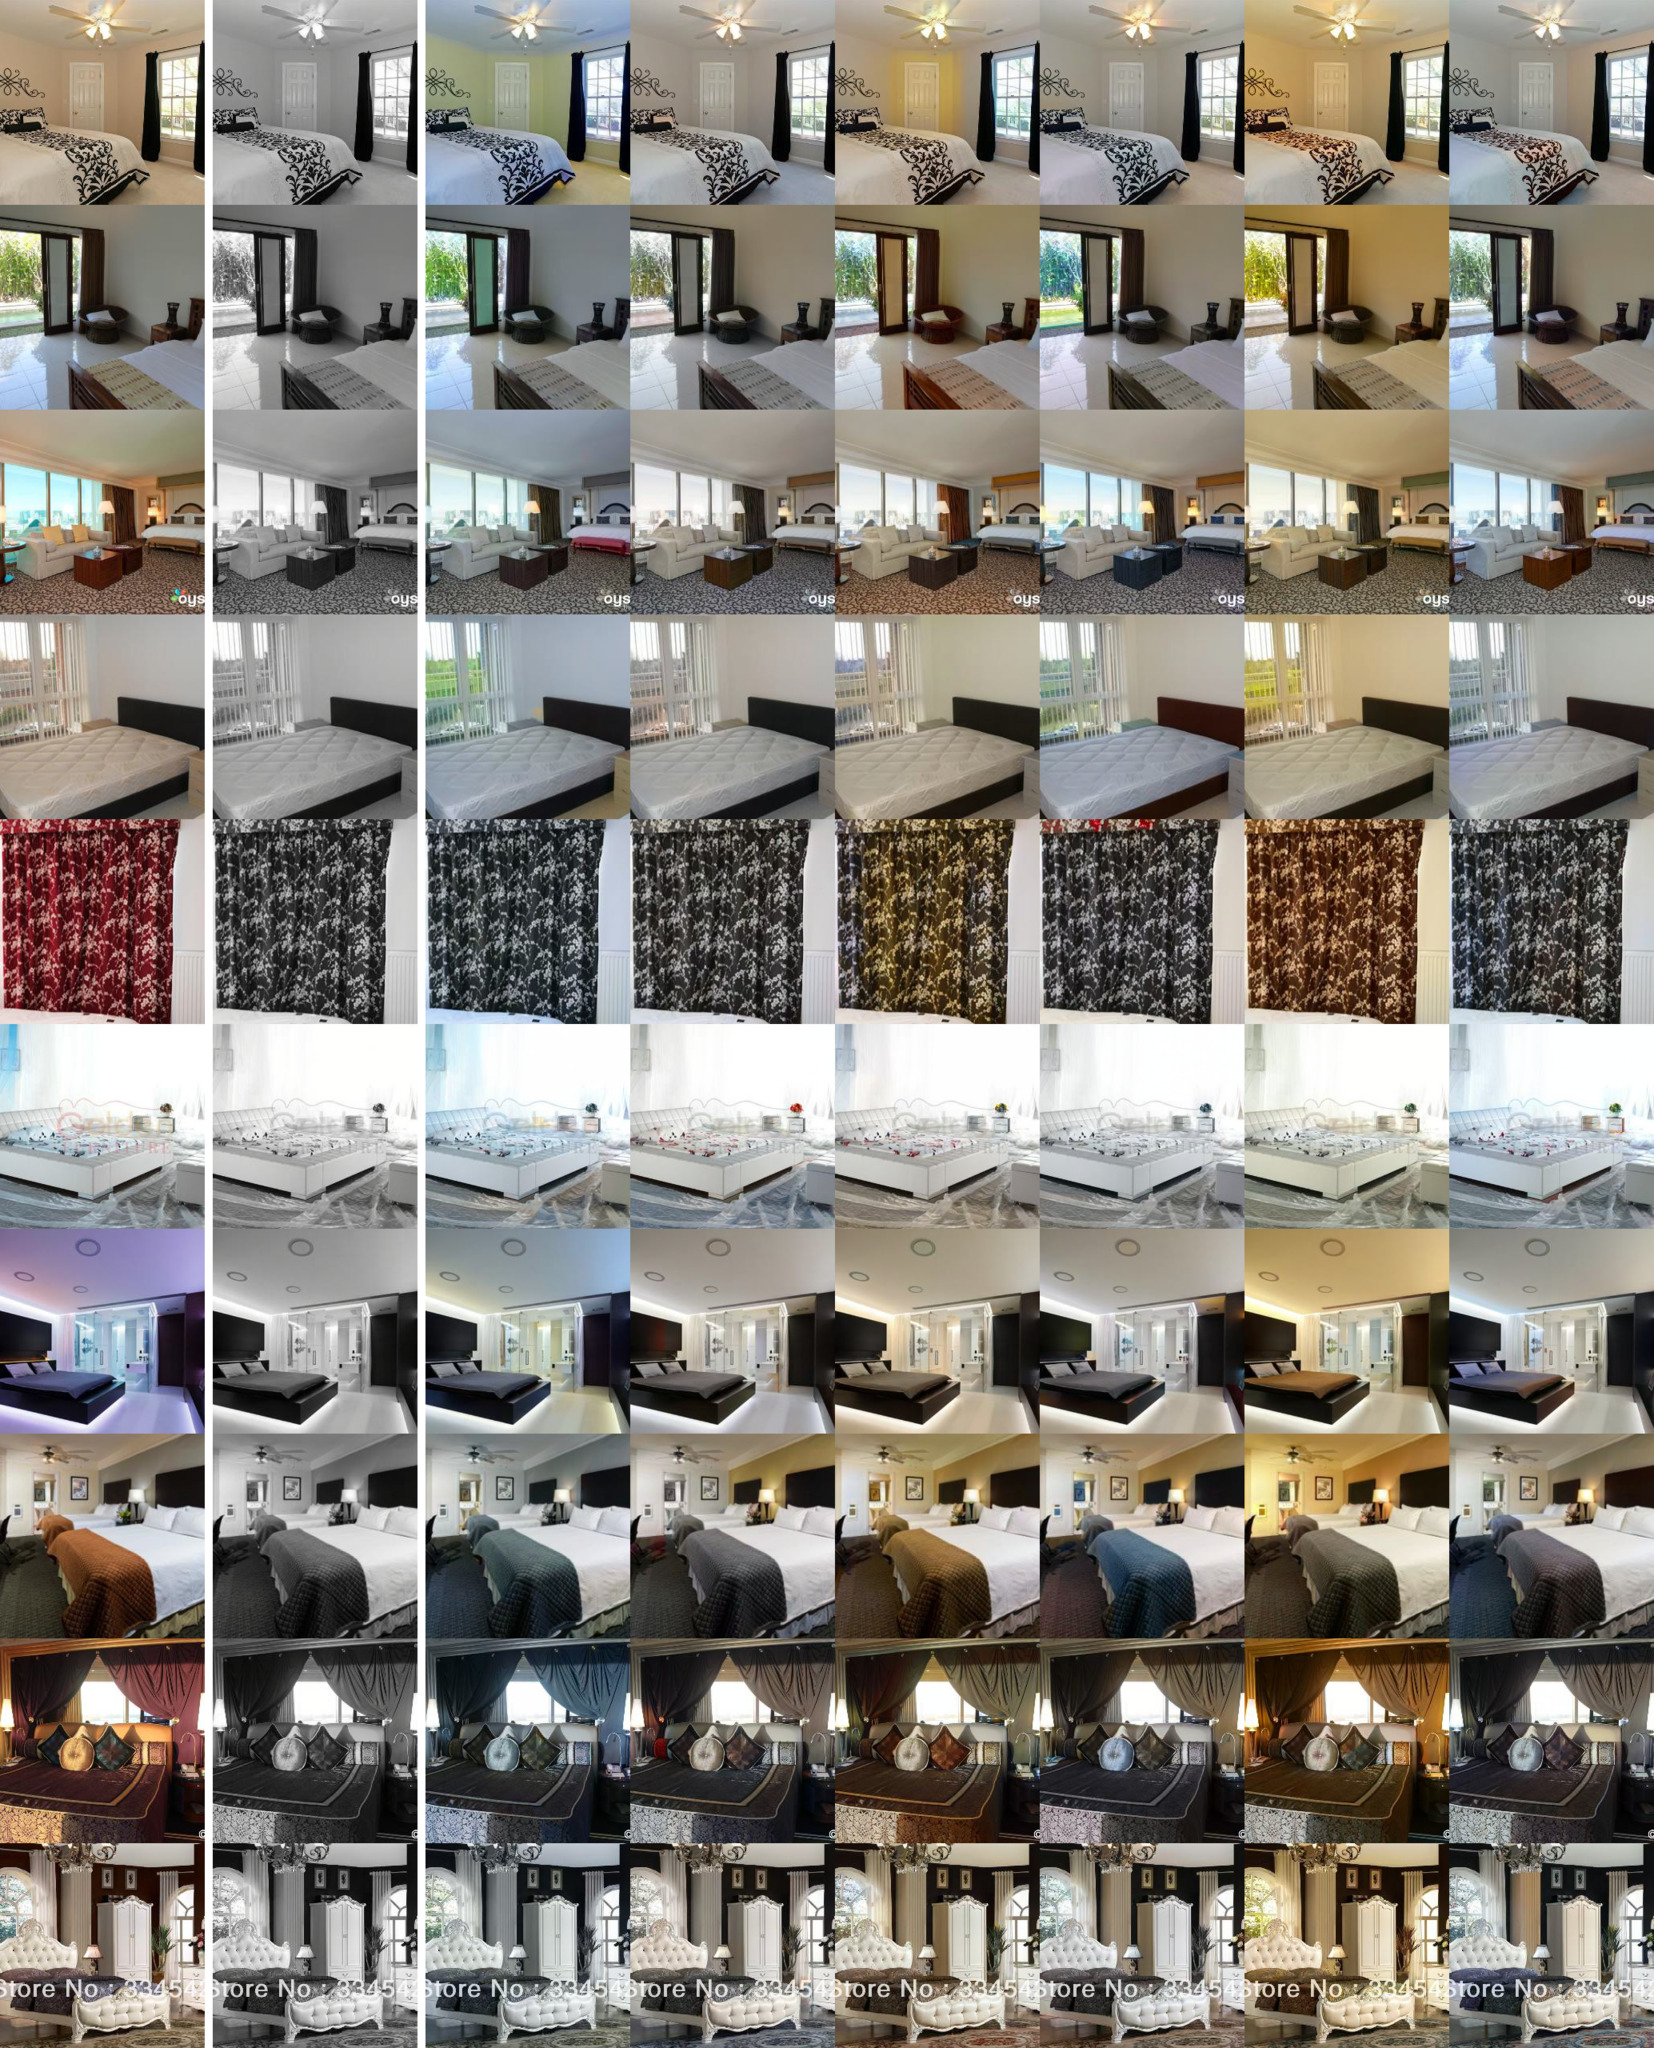
\includegraphics[width=\linewidth]{figures/bedroom_colorization.jpg}
    \caption{Extended colorization results for $256\times 256$ bedroom images.}
    \label{fig:bedroom_colorization}
\end{figure}

\begin{figure}
    \centering
    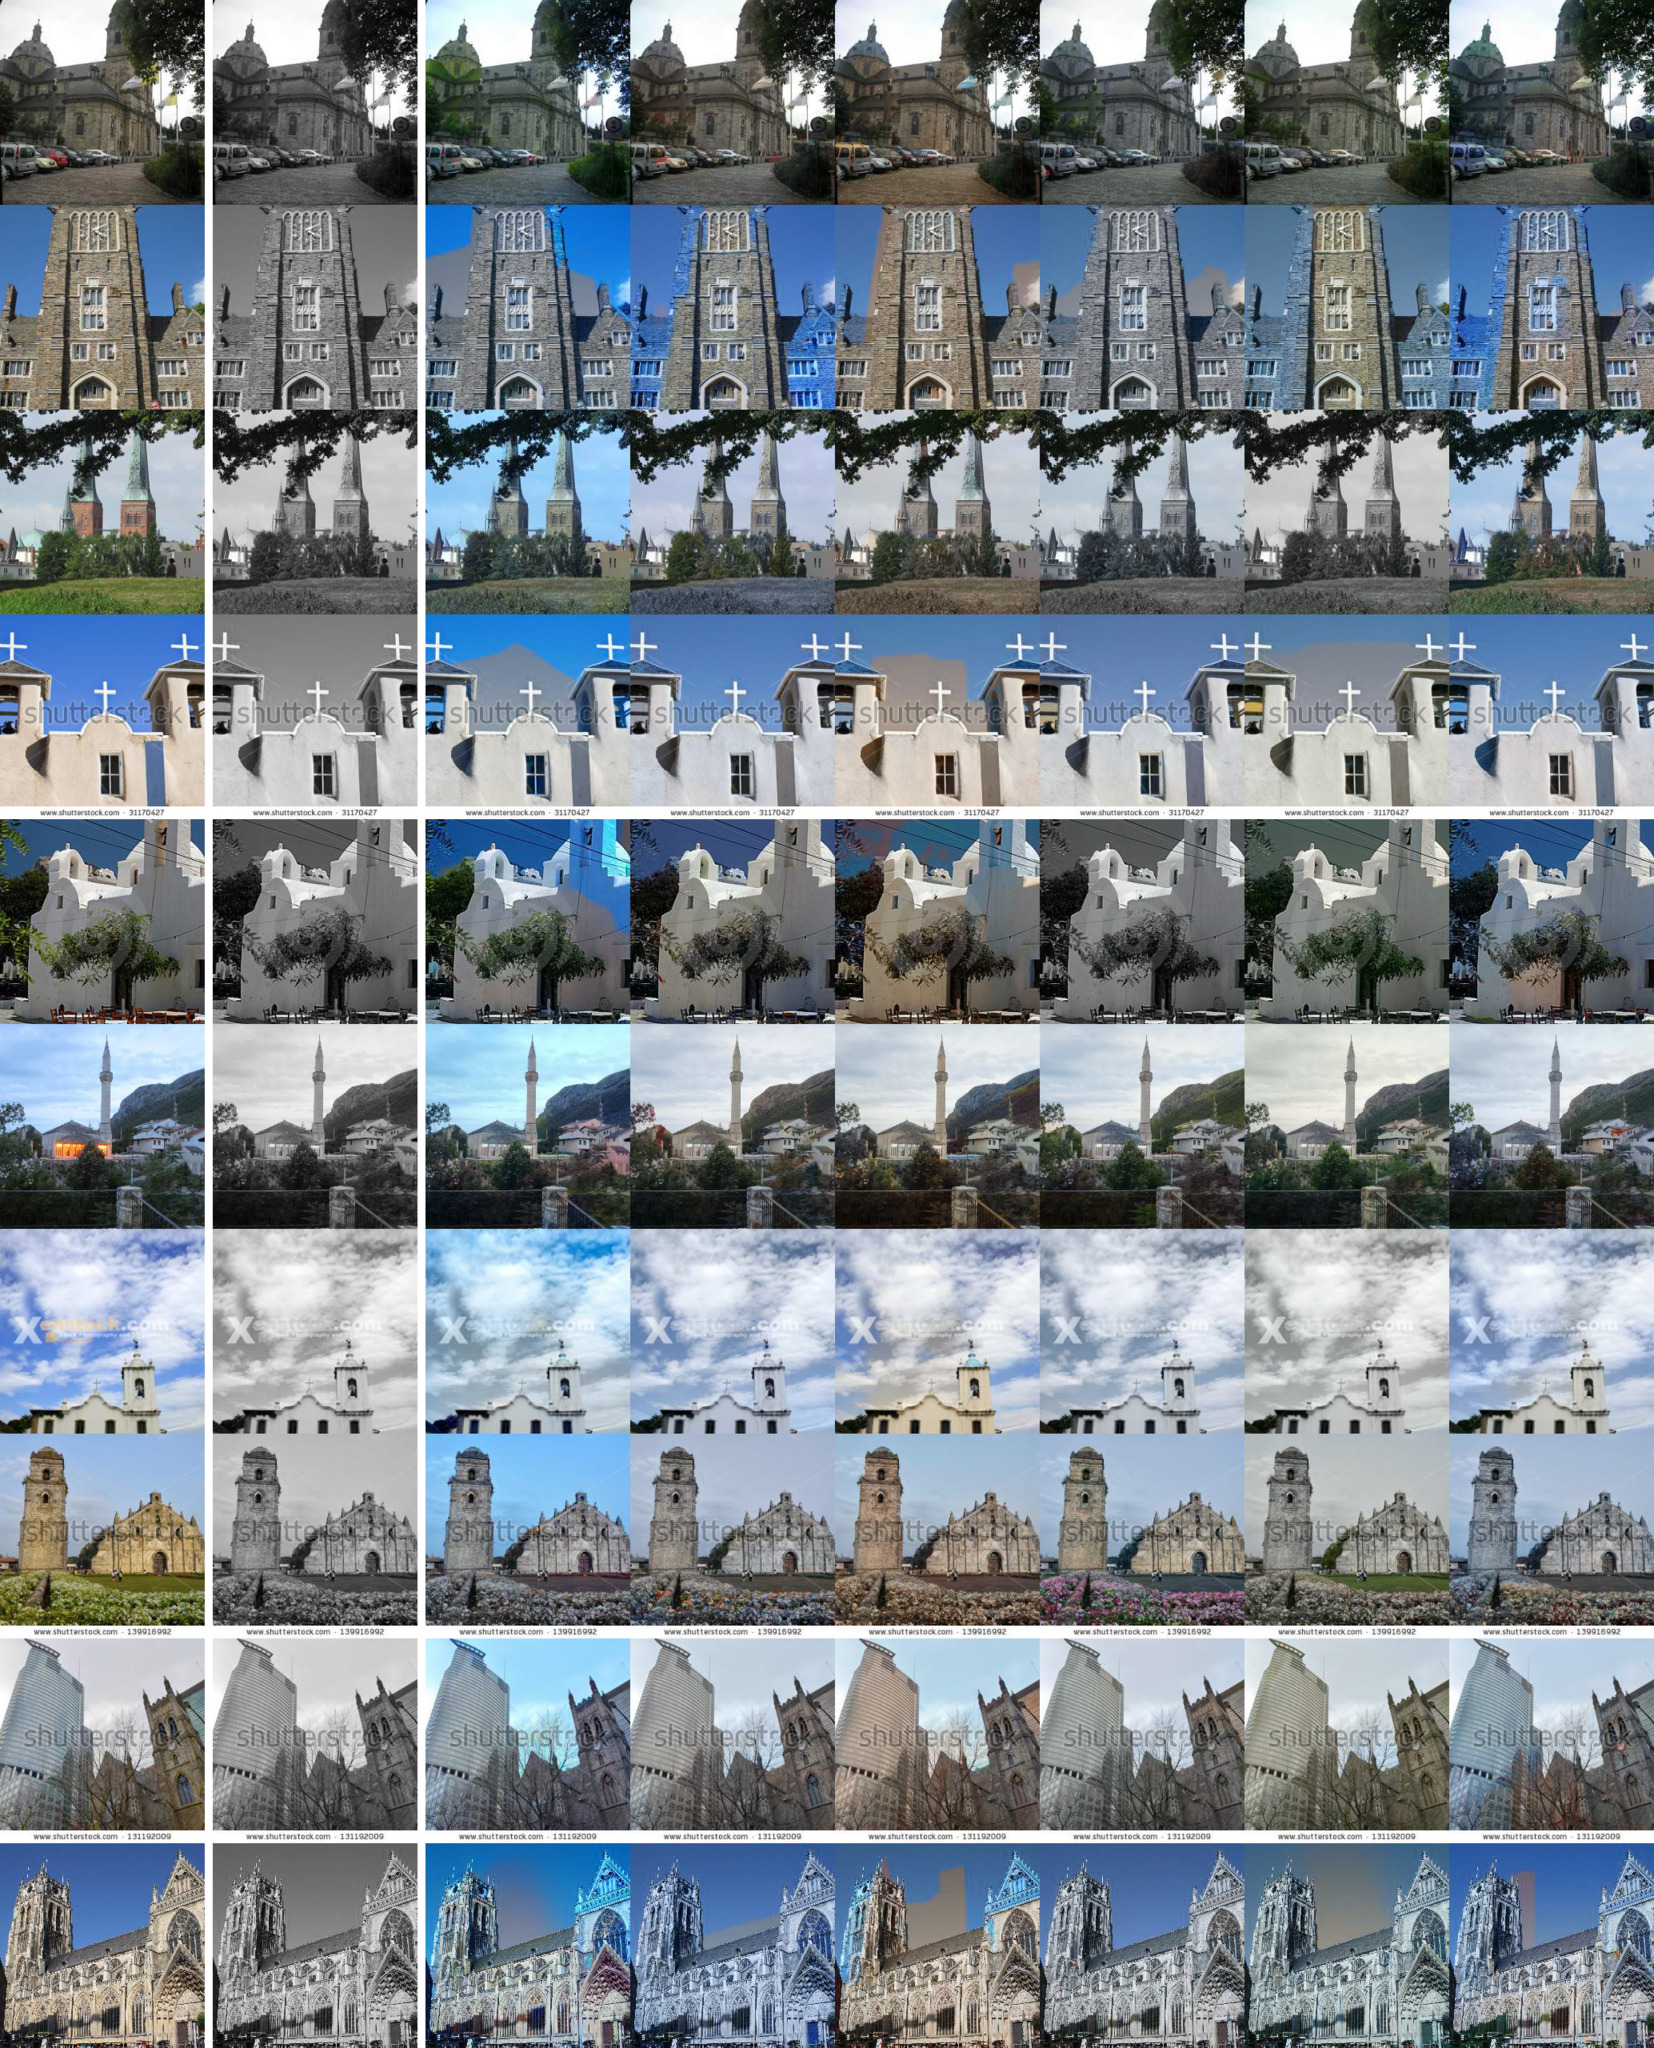
\includegraphics[width=\linewidth]{figures/church_colorization.jpg}
    \caption{Extended colorization results for $256\times 256$ church images.}
    \label{fig:church_colorization}
\end{figure}

We provide an extended set of colorization results in \cref{fig:bedroom_colorization,fig:church_colorization}.